\documentclass[draftcls,onecolumn,12pt]{IEEEtran}
\usepackage[utf8]{inputenc}
\usepackage{framed}
\usepackage[linesnumbered,lined, algoruled]{algorithm2e}
\usepackage{algorithmic,float}
\usepackage{amsmath}
\usepackage{amsthm}
\usepackage{amsfonts}
\usepackage{amssymb}
\usepackage{bm,array}
\usepackage{soul,color}
%\usepackage{epstopdf}
\usepackage[acronym,shortcuts]{glossaries}
\usepackage{graphicx}
\usepackage{graphics}
\usepackage{comment}
\usepackage{setspace}
\usepackage[inline]{enumitem}
\makeglossaries
%%% Glossaries/Acronyms
\DeclareMathOperator\erf{erf}
\newacronym{ae}{AE}{auto encoder}
\newacronym{auc}{AUC}{area under the curve}
\newacronym{ap}{AP}{access point}
\newacronym{ce}{CE}{cross entropy}
\newacronym{cdf}{CDF}{cumulative distribution function}
\newacronym{fa}{FA}{false alarm}
\newacronym{gnss}{GNSS}{global navigation satellite systems}
\newacronym{irlv}{IRLV}{in-region location verification}
\newacronym{kl}{K-L}{Kullback-Leibler}
\newacronym{ls}{LS}{least-squares}
\newacronym{llr}{LLR}{log likelihood-ratio}
\newacronym{los}{LOS}{line of sight}
\newacronym{glrt}{GLRT}{generalized likelihood ratio test}
\newacronym{lssvm}{LS-SVM}{least squares SVM}
\newacronym{md}{MD}{mis-detection}
\newacronym{ml}{ML}{machine learning}
\newacronym{mlp}{MLP}{multy-layer perceptron}
\newacronym{mmse}{MMSE}{minimum mean square error}
\newacronym{mse}{MSE}{mean squared error}
\newacronym[\glslongpluralkey={neural networks}]{nn}{NN}{neural network}
\newacronym{np}{N-P}{Neyman-Pearson}
\newacronym{oclssvm}{OCLSSVM}{one-class least-square \ac{svm}}
\newacronym{pdf}{PDF}{probability density function}
\newacronym{pso}{PSO}{particle swarm optimization}
\newacronym{roc}{ROC}{receiver operating characteristic}
\newacronym{roi}{ROI}{region of interest}
\newacronym{rss}{RSS}{received signal strength}
\newacronym[\glslongpluralkey={support vector machines}]{svm}{SVM}{support vector machine}
\newacronym{ue}{UE}{user equipment}
\expandafter\def\expandafter\quote\expandafter{\quote\setstretch{1}~\\}
% Revisions macro
\usepackage[normalem]{ulem}
\usepackage[user]{zref}
\newcommand{\sot}[1]{}

\newcounter{revc}
\makeatletter \zref@newprop{revcontent}{} \zref@addprop{main}{revcontent}
\zref@newprop{revsec}{} \zref@addprop{main}{revsec}

\newcommand{\revi}[2]{%
\zref@setcurrent{revsec}{\thesection}%
\zref@setcurrent{revcontent}{#2}%
\refstepcounter{revc}%
\label{#1}
\zlabel{#1}%
\uline{#2} }

\newcommand{\revinu}[2]{%
\zref@setcurrent{revsec}{\thesection}%
\zref@setcurrent{revcontent}{#2}%
\refstepcounter{revc}%
\zlabel{#1}%
\label{#1}
#2 }

\newcommand{\revr}[2]{%
\zref@setcurrent{revsec}{\thesection}%
\zref@setcurrent{revcontent}{#2}%
\refstepcounter{revc}%
\zlabel{#1}%
\label{#1} \sot{#2}} \makeatother
\newcommand{\revp}[1]{\zref[revcontent]{#1}}
\newcommand{\zsecref}[1]{\zref[revsec]{#1}}



\newcommand{\ie}{i.e., }
\newcommand{\wrt}{with respect to }
\newcommand{\Exp}[1]{\mathbb{E}\left[#1\right]}
\newcommand{\ai}{\bm{a}^{(i)}}
\newcommand{\A}[1]{\mathcal{A}_#1}

\DeclareMathOperator{\sign}{sign}
\newcommand{\E}{E}
\newtheorem{theorem}{Theorem}
\newtheorem{lemma}{Lemma}
\newtheorem{corollary}{Corollary}

\title{Machine Learning For In-Region Location Verification In Wireless Networks}
\author{Alessandro Brighente, Francesco Formaggio, Giorgio Maria Di Nunzio, \\ and  Stefano Tomasin }
\date{\today}


%\usepackage[autostyle]{csquotes}
\usepackage[backend=biber,style=ieee]{biblatex}
\bibliography{bibliography}


\begin{document}


\maketitle

\sloppy

\begin{abstract}
\Ac{irlv} aims at verifying whether a user is inside a \underline{region of interest (ROI)}, and in wireless networks it can exploit the features of the channel between the user to be verified and the set of trusted access points. As \ac{irlv} is an hypothesis testing problem we can resort to the \ac{np} theorem, when channel statistics are known. By removing the channel knowledge assumption we instead consider \ac{ml} solutions based on either \acp{nn} or \ac{svm} to learn channel features characteristics of the ROI. We show that \ac{ml} approaches are \ac{np}-optimal for sufficiently complex machines and long enough training. For finite training \ac{ml} turns out to be more accurate than then \ac{np} applied on estimated channel statistics. \revi{rev14}{When the channel feature data is available only for the normal scenario (and not for the attack) we resort to one-class classifications, namely through the auto-encoder and one-class \ac{svm}. However,  we prove that they are not equivalent to the  \acf{glrt}, that typically replaces \ac{np} when statistics under only one hypothesis are available. Lastly, we consider  the use of (one-class) classifiers to accelerate the success of a sequence of attacks made from various positions.} Numerical results are provided to support the results in a realistic cellular scenario, including shadowing and fading effects for the channel description.
\end{abstract}

\begin{IEEEkeywords}
Auto-encoder, in-region location verification, machine learning, neural network, support vector machine.
\end{IEEEkeywords}

\glsresetall
\clearpage
\section{Introduction}

Location information without verification gives ample opportunities to attack a service granting system since the location information can be easily manipulated either by tampering the hardware/software reporting the location or by spoofing the \ac{gnss} signal outside the user device. In this context, location verification systems aim at verifying the position of mobile devices in a mobile communication network. These systems can be used to implement location-based granting systems, e.g., location-based access control, media streaming, and social networking, and have applications in sensor networks \cite{Zeng-survey, 8376254, wei2013}, the Internet of Things \cite{7903611}, and geo-specific encryption solutions \cite{quaglia}. In the literature, there are approaches that leverage the features of the wireless channel over which communication occurs. For example, the approach proposed by \cite{yan2016location} uses \ac{rss} to provide the measurement of the distance between the user and other network nodes. \revi{rev3cit}{Moreover, the location verification problem is similar to the  {\em user authentication} problem addressed at the physical layer where channel measurements are processed to verify the identity of the message sender. Examples include the comparison of an estimated channel feature with a  reference channel feature when the noise statistics is known \protect{\cite{Baracca-12}}, or learning strategies when the channel statistics are unknown \protect{\cite{7398138}} (see also \protect{\cite{7270404}} for a survey).}

In this work, we focus on \ac{irlv} that aims at verifying whether a user is inside a specific \ac{roi} by exploiting the features of the channel between the user to be verified and a set of trusted \acp{ap} \cite{Zeng-survey}. In this regard, distance bounding techniques with rapid exchanges of packets between the verifier and the prover have been proposed in \cite{Brands}. Different solutions use radio-frequency and ultrasound signals \cite{Sastry} or anchor nodes and increasing transmit power by the sender \cite{Vora}. More recently, a delay-based verification technique leveraging geometric properties of triangles, which prevents an adversary from manipulating measured delays, has been proposed in \cite{7145434}.  
%
Some of the proposed techniques partially neglect wireless channel phenomena (such as shadowing and fading) that make the estimation of distance measurements through the wireless communication signal problematic \cite{Brands,Sastry,Vora}. Other approaches assume specific channel statistics \cite{quaglia} that may be not accurate due to changing environment conditions, their dependency on unknown parameters, or the use of advanced signal processing techniques by the attacker. Indeed, if the statistics of the channels of links to devices both inside and outside the \ac{roi} are known to the network infrastructure, the optimal solution for \ac{irlv} is given by the \ac{np} theorem \cite{Cover-book} that provides the most powerful test for a given significance level. 

When the knowledge of the channel statistics is not available, a two-step solution would be to a) estimate the channel statistics and b) apply the \ac{np} theorem on the estimated statistics. However, as we also confirm in this paper, this approach may not be accurate. Alternatively, \ac{ml} techniques can be used to exploit the available training data and to optimize directly the decision process rather than going through the two-step solution. For example, in \cite{xiao-2018} no assumption is made on the channel model and logistic regression has been proposed as an alternative to hypothesis testing. In \cite{tian2015robust}, the objective is to locate the user inside a building and a multi-class classification problem is solved via \ac{svm}. Nevertheless, neither \cite{xiao-2018}  nor \cite{tian2015robust} compare the performance of their \ac{ml} approaches with the theoretical optimum \ac{np} criterion.

In this paper, we remove the channel knowledge assumption and study two \ac{ml} solutions based on \acp{nn} and \ac{svm} to learn channel features of the \ac{roi}. We investigate two loss functions for the \ac{mlp} design: the \ac{ce} and the \ac{mse}; while we study the \ac{ls} implementation of the \ac{svm}. We show that these two approaches are \ac{np}-optimal for sufficiently complex machines as well as sufficiently large training data. Moreover, for a limited training dataset, the \ac{ml} approach turns out to be more accurate than \ac{np} applied on estimated channel statistics. 

Two specific security issues are then addressed. Firstly, the attacker can select the location for the attack and its statistics \hl{non mi e' chiaro its statistics a cosa faccia riferimento} can be modified. We explore the one-class classification problem both under the knowledge of legitimate channel statistics and by a \ac{ml} approach, and we conclude that conventional \ac{ml} solutions based on both the \ac{ae} and one-class \ac{svm} do not coincide with the \ac{glrt}, even under asymptotic training  conditions. \revi{rev11a}{The obtained asymptotic results are applicable also to elaborate ML solution, such as deep learning NNs, that can still be seen as parametric functions, although more complex than conventioanl NNs.}Secondly, advanced attacks based on the use of \ac{ml} techniques to select the positions of attack by the attacker are considered. Numerical results are provided to support the results in a realistic network scenario, including shadowing and fading effects for the channel. We show that in a simple scenario a simple \ac{nn} and a relatively small training dataset already provide close-to-optimal performance; then, we assess the one-class \ac{irlv} approach as well as the advanced attack strategy based on \ac{ml}. \revi{WiFi}{Indeed, while at the moment most literature has focused on WiFi or IoT applications for \ac{irlv}, positioning is a relevant feature for 5G and beyond cellular systems, and as reference example we consider a cellular scenario in this paper.}

The contributions of this paper are summarized hereby:
\begin{itemize}
    \item We propose a  physical layer-based \ac{irlv} system exploiting \ac{ml} techniques to perform hypothesis testing;
    \item We show that two-class classification \ac{ml} techniques provide the most powerful test for a given significance level, as the \ac{np} test;
    \item We compare different \ac{ml} techniques and show how these can be exploited to implement both \acp{irlv} and efficient attacks.
\end{itemize}

The rest of the paper is organized as follows. Section II introduces the system model for the \ac{irlv} problem, detailing the channel model and summarizing the \ac{np} theorem under the knowledge of channel statistics. Section III describes the considered \ac{ml} approaches for \ac{irlv}, namely the \ac{mlp} \ac{nn} and the \ac{svm}, with their design approaches based on \ac{mse} or \ac{ce} for the \ac{nn}, and on  \ac{ls} for \ac{svm}. In Section IV, we propose the one-class classification approach where only the channel statistics for locations inside the \ac{roi} are used for training. Both the the \ac{ae} \ac{nn} and the \ac{oclssvm} are considered and their performance is compared with the \ac{glrt} test. Advanced attack strategies based on the use of \ac{ml} by the attacker are proposed in Section V. Numerical results comparing the various techniques are shown and discussed in Section VI. Lastly, the main conclusions are outlined in Section VII.

The following notation is used throughout the paper: bold letters $\bm{x}$ refer to vectors, whereas capital bold letters $\bm{H}$ refer to matrices, $\mathbb{E}[x]$ denotes the expectation of random variable $x$, $(\cdot)^T$ denotes the transpose, $\mathbb P[A]$ denotes the probability of event $A$, and $\ln(x)$ denotes the natural base logarithm of $x$.

\section{System Model}

\begin{figure}
    \centering
    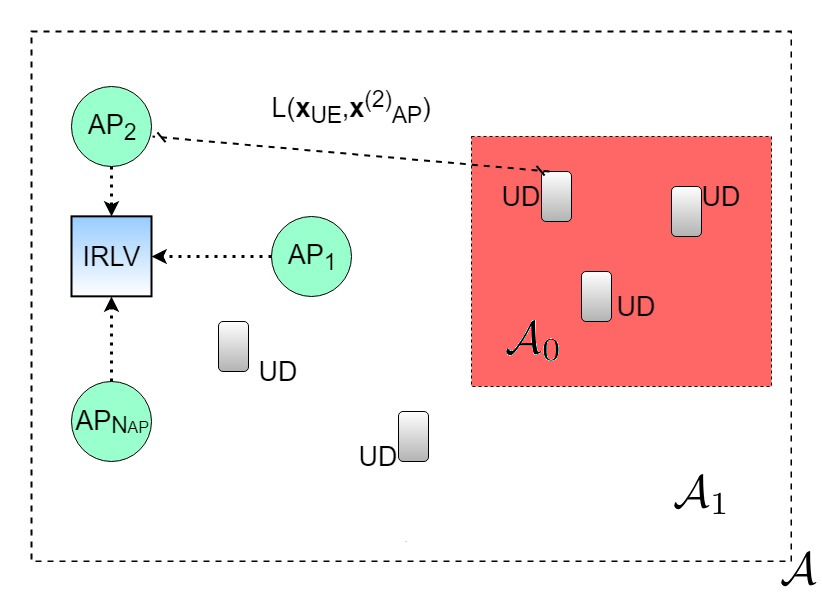
\includegraphics[width=0.6\columnwidth]{irlv.jpg}
    \caption{The considered \ac{irlv} scenario.}
    \label{fig1}
\end{figure}

In Fig. \ref{fig1}, we consider a cellular system with $N_{\rm AP}$ \acp{ap} covering the area $\mathcal{A}$ over a plane. We propose a \ac{irlv} system to determine if a \ac{ue} is transmitting from within an {\em authorized} \ac{roi} $\mathcal{A}_0$ inside  $\mathcal{A}$. we define the complementary region to the \ac{roi} as $\mathcal{A}_1=\mathcal{A} \setminus \mathcal{A}_0$. The authentication process exploits the location dependency of the features of the channel between the \ac{ue} and the \acp{ap}. \revi{revPHASE}{As an exmple of \ac{irlv} based on physical channel features, we consider here a narrowband transmission and choose as feature the power attenuation. This is in line with various works in the literature \protect{\cite{boh}}. Indeed, other features can also be exploited, such as the phase or the wideband impulse response: the proposed ML techniques readily applied also to this cases as we do not make special assumptions on the channel model for their design and analysis.}

The exploitation of the channel features is obtained by letting the \ac{ue} transmit a signal with fixed power $P_{\rm tx}$, known at the \acp{ap}, from which the \acp{ap} can estimate the received power and obtain a measure of the attenuation incurred by the channel. We assume that the attenuation estimation is perfect, i.e., not affected by noise or interference: this can be achieved by using a sufficiently long signal.



\subsection{Channel Model}\label{sec:chMod}

When the \ac{ue} transmits with power $P_{\rm tx}$, the received power at the $n^{\rm th}$ \ac{ap} is
\begin{equation}\label{eq: rec pow}
    P_{\rm rc}^{(n)}= \frac{P_{\rm tx}}{a^{(n)}},
\end{equation}
where $a^{(n)}$ is the attenuation incurred over the channel between the \ac{ue} and the \ac{ap} $n$. The channel model for path-loss and shadowing is derived from \cite{3gpp}. The attenuation coefficient includes the effects of path-loss, shadowing and fading. In particular, by assuming Rayleigh model for fading we have 
\begin{equation}
    \sqrt{a^{(n)}} \sim \mathcal{N}\left(0,\sigma_{a,n}^2\right),
\end{equation}
where $(\sigma_{a,n}^2)_{dB} =  {P_{\rm PL}^{(n)}}  + s$ accounts for the path-loss and shadowing components, $(P_{\rm PL}^{(n)})$ is the path-loss coefficient in dB, and $s \sim \mathcal{N}(0,\sigma_s^2)$ is the shadowing component.

%Both path-loss and shadowing models are  derived from \cite{3gpp}. 
In particular, let us denote as $\bm{x}_{\rm AP}^{(n)} =(X_{\rm AP}^{(n)},Y_{\rm AP}^{(n)})$ the position of  \ac{ap} $n= 1, \ldots, N_{\rm AP}$. For a \ac{ue} located at $\bm{x}_{\rm UE}=(X_u,Y_u)$, its distance from \ac{ap} $n$ is $L(\bm{x}_{\rm UE},\bm{x}_{\rm AP}^{(n)}) = \sqrt{(X_{\rm AP}^{(n)}-X_u)^2+(Y_{\rm AP}^{(n)}-Y_u)^2}$. 

\revi{WiFi2}{Here we focus on a cellular communication scenario as a reference model for performance evaluation. However, the proposed \ac{irlv} technique can also be applied to wireless local area networks (WLANs) and IoT scenarios.} For the path-loss, we consider two scenarios: \ac{los} and non-\ac{los}. For a \ac{los} link, the path-loss in dB is modelled as
\begin{equation}\label{eq:los}
    P_{{\rm PL},{\rm LOS}}\left(L(\bm{x}_{\rm UE},\bm{x}_{\rm AP}^{(n)})\right) = 10 \nu \log_{10}\left(\frac{f 4\pi L(\bm{x}_{\rm UE},\bm{x}_{\rm AP}^{(n)})}{c}\right),
\end{equation}
where $\nu$ is the path-loss coefficient, $f$ is the carrier frequency and $c$ is the speed of light. 
For a  non-\ac{los} link, the path-loss coefficient in dB is defined as
\begin{equation}\label{eq:nlos}
    P_{{\rm PL}, {\rm NLOS}}\left(L(\bm{x}_{\rm UE},\bm{x}_{\rm AP}^{(n)})\right) = 40\log_{10}\left (\frac{L(\bm{x}_{\rm UE},\bm{x}_{\rm AP}^{(n)})}{10^3}\right ) + 21\log_{10}\left(\frac{f}{10^6}\right) + 80.
\end{equation}

The shadowing parameter $s$ is zero-mean Gaussian distributed with power $\sigma^2_s$. Moreover, the shadowing parameters of two \acp{ue} located at positions $\bm{x}_i$ $\bm{x}_j$ and transmitting to the same \ac{ap} have correlation $\sigma_s^2e^{-\frac{L(\bm{x}_i,\bm{x}_j)}{d_c}}$, where $d_c$ is the shadowing decorrelation distance \underline{\cite[Chapter 2.7]{goldsmith2005}}. 

Path-loss and shadowing are assumed to be time-invariant, while the fading component is independent at each attenuation estimate. 


\subsection{\ac{irlv} With Known Channel Statistics}\label{sec:auth}

The \ac{irlv} problem can be seen as a hypothesis testing between the two hypotheses (events):
\begin{itemize}
    \item $\mathcal{H}_0$: the \ac{ue} is transmitting from area $\mathcal{A}_0$;
    \item $\mathcal{H}_1$: the \ac{ue} is transmitting from area $\mathcal{A}_1$.
\end{itemize}
This is also denoted as a two-class classification problem. Given vector $\bm{a} = [a^{(1)}, \ldots, a^{(N_{\rm AP})}]$ collecting the attenuation estimates at all the \acp{ap}, we aim  at determining the most likely hypothesis in order to perform \ac{irlv}. While a few measurements of path-loss would allow, by triangulation, to establish the exact position of the \ac{ue}, both shadowing and fading make the \ac{irlv} more problematic and in general prone to errors. 

\revi{avg_1}{We also consider the scenario in which the \ac{ap} averages out fading by measuring $N_{\rm avg}$ received power realizations. The feature vector in this case is $\bm{a}_{\Sigma} = [a^{(1)}_{\Sigma}, \ldots, a^{(N_{\rm AP})}_\Sigma]$, where} 
\begin{equation}
\label{eq:avg}
a^{(n)}_{\Sigma} = \frac{1}{N_{\rm avg}}\sum_{j=1}^{N_{\rm avg}} a^{(n)}.
\end{equation} 
\revi{avg_2}{Note that each element of the sum in \eqref{eq:avg} is a different fading realization with the same shadowing power. We thus model the situation in which the user is standing still for $N_{\rm avg}$ measurement periods and the  \ac{ap} exploits all the measurements to mitigate the fading effects.}

Let $\mathcal H \in  \{\mathcal{H}_0, \mathcal{H}_1\}$ be the effective location of the \ac{ue}, and $\hat{\mathcal H} \in  \{\mathcal{H}_0, \mathcal{H}_1\}$ the decision taken at the \acp{ap}. We have two possible errors: \acp{fa}, which occur when the \ac{ue}  is classified as outside the \ac{roi}, while being inside it, and \acp{md}, which occur when the \ac{ue}  is classified as inside the \ac{roi}, while being outside of it. We indicate the probability of \ac{fa} as $P_{\rm FA} =P(\hat{\mathcal H} = \mathcal H_1 | \mathcal H = \mathcal H_0)$ and the  probability of \ac{md} as $P_{\rm MD}=P(\hat{\mathcal H} = \mathcal H_0 | \mathcal H = \mathcal H_1)$. 
%
Let $p(\bm{a}|\mathcal{H}_i)$ be the probability of observing the vector $\bm{a}$ given that $\mathcal{H} = \mathcal{H}_i$. The \ac{llr} for the considered hypothesis is defined as 
\begin{equation}\label{eq:lr}
    {\mathcal M}(\bm{a})=\ln \frac{p(\bm{a}|\mathcal{H}_0)}{p(\bm{a}|\mathcal{H}_1)}.
\end{equation}
According to the \ac{np} theorem, the most powerful test is obtained by comparing $\mathcal{M}(\bm{a})$ with a threshold value $\Lambda$, i.e., obtaining the test function
\begin{equation}
\label{eq:oneClassDec}
f^*(\bm{a}) =
\begin{cases}
-1 &\text{if } {\mathcal M}(\bm{a}) \geq \Lambda, \\
1 & \text{if } {\mathcal M}(\bm{a}) < \Lambda.
\end{cases}
\end{equation}
\revi{lambda}{The value $\Lambda$ is a parameter which grants a certain significance level, meaning the probability of rejecting the null hypothesis when it is true ($P_{\rm FA}$). The parameter $\Lambda$ shall hence be chosen according to the \ac{fa} performance that we require by the system and its value must be computed by trial and error. The \ac{np} test hence guarantees that, by implementing hypothesis testing as in (\ref{eq:oneClassDec}), for the selected $P_{\rm FA}$ value, the resulting $P_{\rm MD}$ is minimum and hence optimal.}

\subsection{Example of \ac{np} Test}\label{sec:los}
\begin{figure}
    \centering
    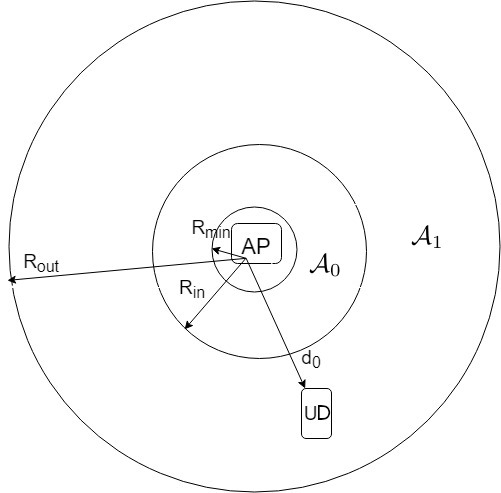
\includegraphics[width=0.5\columnwidth]{simpleScen.jpg}
    \caption{Simplified scenario with a single \ac{ap} located at the center of a circular \ac{roi}.}
    \label{fig:simpScen}
\end{figure}
\revi{simpleScen}{We provide here an example of an application of the \ac{np} theorem to the simple scenario of Fig. \ref{fig:simpScen}, where area $\mathcal{A}$ is a circle with radius $R_{\rm out}$ ans \ac{roi} $\mathcal{A}_{0}$ is an annulus concentric to the overall area with larger radius $R_{\rm in}$ and smaller radius $R_{\rm min}$. A single \ac{ap} ($N_{\rm AP} =1$) is located at the \ac{roi} center and a \ac{ue} is transmitting from distance $d$. We consider two models: a) \emph{fading scenario}, which includes path-loss and fading, and b) \emph{shadowing scenario} which includes path loss and shadowing. In both cases we consider the \ac{los} scenario for path-loss.}
\revi{simpleScen2}{In order to compute $p(a|\mathcal{H}_i)$ we first observe that the probability of incurring in an attenuation $a$ for a user located inside the \ac{roi} is given by the total probability law}
\begin{equation}\label{eq:prc}
p(a|\mathcal{H}_0) = \int_{0}^{R_{\rm in}} p\left( \frac{P_{\rm tx}}{a} | d = d_0\right)p(d_0| d_0 \in \mathcal{A}_0) \, dd_0,    
\end{equation}
\revi{simpleScen2_1}{where $p(d_0| d_0 \in \mathcal{A}_0)$ is the probability of the \ac{ue} transmitting from distance $d_0$ inside the \ac{roi}. Assuming that \ac{ue} position is uniformly distributed in the whole area we have} \hl{attenzione PL in dB!}
\begin{equation}\label{eq:a0}
p(d_0| d_0 \in \mathcal{A}_0) =
\begin{cases}
\frac{2 d_0}{R_{\rm in} ^ 2-R_{\rm min}^2} \, \, d_0 \in [R_{\rm min}, R_{\rm in}], \\
0 \, \, d_0 > R_{\rm in}
\end{cases}
\end{equation}
\revi{simpleScen2_2}{whereas}
\begin{equation}\label{eq:a1}
p(d_0| d_0 \in \mathcal{A}_1) =
\begin{cases}
0 \, \, d_0 \leq R_{\rm in},\\
\frac{2 d_0}{R ^ 2- R_{\rm in} ^2} \, \, d_0 \in (R_{\rm in},R].
\end{cases}
\end{equation}
\subsubsection{Fading scenario}
\revi{simpleScen3} {Assuming spatially uncorrelated Rayleigh fading the received power at the \ac{ap} given a user located at distance $d$ is exponentially distributed with mean $P_{{\rm PL},{\rm LOS}}(d)$ given by (\ref{eq:los}). Hence from (\ref{eq:a0}) we have}

\begin{equation}\label{eq:fading}
    p(a|\mathcal{H}_0) = 
    \frac{2}{R_{\rm in}^2-R_{\rm min}^2}\int_{R_{\rm min}}^{R_{in}} 10^{P_{{\rm PL},{\rm LOS}}(d_0)/10} \exp\left(-10^{P_{{\rm PL},{\rm LOS}}(d_0)/10} \frac{P_{\rm tx}}{a}\right)d_0 \, dd_0,
\end{equation}
\revi{simpleScen3_1}{whereas from (\ref{eq:a1}) we have}
\begin{equation}\label{eq:fading2}
    p(a|\mathcal{H}_1) = 
    \frac{2}{R^2-R_{\rm in}^2}\int_{R_{\rm in}}^R 10^{P_{{\rm PL},{\rm LOS}}(d_0)/10} \exp\left(-10^{P_{{\rm PL},{\rm LOS}}(d_0)/10} \frac{P_{\rm tx}}{a}\right)d_0 \, dd_0,
\end{equation}
\revi{simpleScen3_2}{By computing integrals for path-loss coefficient $\nu = 2$ the \ac{llr} is} 
\begin{equation}\label{eq:llr1}
   \mathcal{M}(a) =
   \ln\left(\frac{R^2-R_{\rm min}^2}{R_{\rm in}^2-R_{\rm in}^2}\frac{\mathcal{V}(R_{\rm min},a)-\mathcal{V}(R_{\rm in},a)}{\mathcal{V}(R_{\rm in},a)-\mathcal{V}(R,a)}\right),
\end{equation}
\revi{simpleScen3_2_1}{where}
\begin{equation}
\mathcal{V}(d_0,a) = \exp\left(-\frac{P_{\rm tx}}{a}\left(\frac{4 \pi f_0 d_0}{c}\right)^2\right) \left(\frac{P_{\rm tx}}{a}\left(\frac{4 \pi f_0 d_0}{c}\right)^2+1\right) .   
\end{equation}

\revi{simpleScen3_3}{For $\nu=3$ we have instead}
\begin{multline}\label{eq:llr2}
 \mathcal{M}(a) =
 \ln\left(\frac{R^2-R_{\rm in}^2}{R_{\rm in}^2-R_{\rm min}^2}\frac{\Gamma\left(\frac{5}{3},\frac{P_{\rm tx}}{a}\left(\frac{4 \pi f_0}{c}\right)^3 R_{\rm min}^3\right)-\Gamma\left(\frac{5}{3},\frac{P_{\rm tx}}{a}\left(\frac{4 \pi f_0}{c}\right)^3 R_{\rm in}^3\right)}{\Gamma\left(\frac{5}{3},\frac{P_{\rm tx}}{a}\left(\frac{4 \pi f_0}{c}\right)^3 R_{\rm in}^3\right)-\Gamma\left(\frac{5}{3},\frac{P_{\rm tx}}{a}\left(\frac{4 \pi f_0}{c}\right)^3 R^3\right)}\right),
\end{multline}
\revi{simpleScen3_4}{where $\Gamma(\gamma,b)= \int_{b}^{\infty}t^{\gamma-1}e^{-t} dt$ is the incomplete gamma function.}    

\subsubsection{Shadowing scenario}
\revi{simpleScen4}{Assuming spatially uncorrelated shadowing the received power is distributed in the logarithmic domain as a Gaussian random variable with mean value given by the path-loss (\ref{eq:los}) and variance $\sigma_s^2$. Considering (\ref{eq:prc}) the probability of incurring an attenuation $a$ in hypothesis $\mathcal{H}_0$ is given by}
\begin{equation}\label{eq:sh}
   p(a|\mathcal{H}_0) = 
    \frac{2}{R_{\rm in}^2-R_{\rm min}^2}\int_{R_{\rm min}}^{R_{\rm in}} \exp\left(-\frac{1}{2}\frac{\left(\frac{P_{\rm tx}}{a}+10\nu\log_{10}\left(\frac{4 \pi f_0 d_0}{c}\right)\right)^2}{\sigma_s^2}\right) d_0 \, d d_0, 
\end{equation}
\revi{simpleScen4_1}{whereas in hypothesis $\mathcal{H}_1$}
\begin{equation}\label{eq:sh1}
    p(a|\mathcal{H}_1) = 
    \frac{2}{R^2-R_{\rm in}^2}\int_{R_{\rm in}}^R \exp\left(-\frac{1}{2}\frac{\left(\frac{P_{\rm tx}}{a}+10\nu\log_{10}\left(\frac{4 \pi f_0 d_0}{c}\right)\right)^2}{\sigma_s^2}\right) d_0 \, d d_0 .
\end{equation}
\revi{simpleScen4_2}{By solving the integrals in (\ref{eq:sh}) and (\ref{eq:sh1}) we obtain the \ac{llr}}
\begin{equation}\label{eq:llr3}
    \mathcal{M}(a) = \ln\left(\frac{R^2}{R_{\rm in}^2} \frac{\mathcal{T}(R_{\rm in})-\mathcal{T}(R_{\rm min})}{\mathcal{T}(R)-\mathcal{T}(R_{\rm in})}\right),
\end{equation}
\revi{simpleScen4_3}{where }
\begin{equation}
    \mathcal{T}(d_0) = \erf\left( \frac{\frac{100 \nu^2}{\sigma_s^2}\ln(d_0)-\ln^2(10)+\frac{\frac{P_{\rm tx}}{a} 10 \nu \ln(10)}{2\sigma_s^2}}{\sqrt{1/2\sigma_s^2}10\nu\ln(10)}\right),
\end{equation}
\revi{simpleScen4_4}{ and $\erf(x)= \frac{2}{\sqrt{\pi}}\int_0^x e^{-t^2} dt$ is the error function.}

\revi{llrComp}{We notice however that the obtained functions are easily computed for a single \ac{ap} and spatially uncorrelated fading and shadowing. In more complicated scenarios including spatially correlated channels and multiple \acp{ap} the probabilities of incurring in a certain attenuation in the two hypotheses would not have a simple solution, making the implementation of \ac{np} test problematic. We thus propose to implement the \ac{irlv} hypothesis testing by \ac{ml} approaches, which do not require the a-priori knowledge of the probability density functions.}

\subsection{Estimated Distance Approach} \label{seccomp}
\revi{literature_1}{In order to compare our approach with existing \ac{irlv} solutions, we consider the the \ac{mmse} approach on estimated distance  \cite{li2010security}. From the measured attenuation, first the distance of the \ac{ue} from the \ac{ap} is estimated by inverting the path-loss models. Then the \ac{ue} position is estimated by solving 
}
	\begin{align}
 \hat{\bm x}_{\rm UE} =  \underset{\bm x}{\arg \min} \sum_{n=1}^{N_{\rm AP}} \left(L(\bm{x},\bm{x}_{\rm AP}^{(n)}) - L(\bm{x}_{\rm UE},\bm{x}_{\rm AP}^{(n)}) \right)^2,\label{probmindist}
\end{align}
\revi{literature_2}{Let $\mathcal B_0$ be the set of points of the border of $\mathcal A_0$. Then measure the  distance of the UE from the  border of $\mathcal{A}_0$ as $d = \min_{\bm{x} \in \mathcal{B}_0} \pm||\hat{\bm x}_{\rm UE} - \bm{x}||$,  where the sign is negative if $\hat{\bm x}_{\rm UE} \in \mathcal A_0$, and positive otherwise. Lastly, $d$ is compared with a suitable threshold $d_0$, chosen in order to achieve desired FA or MD probability, and the test can be written as
}

\begin{equation}
\hat{\mathcal{H}}_{\rm MMSE} = 
\begin{cases}
\mathcal{H}_0 \quad \text{if } d < d_0 \\
\mathcal{H}_1 \quad {\rm otherwise}.
\end{cases}
\end{equation}

\revi{literature_3}{Note that the MSE (\ref{probmindist}) is not the optimal performance metric, since the error on position is not Gaussian. Moreover, this approach requires the knowledge of the path-loss model (including the possibility to distinguish LOS and non-LOS scenarios), which is quite unrealistic in a real deploymenet. Indeed, most of the literature simply assume the perfect knowledge of the \ac{ue}-\ac{ap} distance.}



\section{\Ac{irlv} by Machine Learning Approaches}\label{sec:irlvML}

The application of the \ac{np} theorem requires the knowledge of the conditional channel statistics $p(\bm{a}|\mathcal{H}_i)$ at the \acp{ap}, which can be hard to obtain also because a-priori assumptions on their expressions may be quite unrealistic. Therefore, we propose to use a \ac{ml} approach operating in two phases:
\begin{itemize}
    \item {\em Learning phase}: the \ac{ap} collects attenuation vectors from a trusted \ac{ue} moving both inside and outside the \ac{roi}, while the \ac{ue} reports its position to the \acp{ap}. In this way, the \acp{ap} can learn the behaviour of the attenuation in both regions $\mathcal A_0$ and $\mathcal A_1$.
    \item {\em Exploitation phase}: the \ac{ap} verifies the location of an un-trusted \ac{ue} by the attenuation's estimate using the data acquired in the learning phase. 
\end{itemize}

\revi{supervised}{As in the learning phase the trusted \ac{ue} reports to the \ac{ap} its position, we can assign true labels to all the collected attenuation vectors in this phase and therefore train the \ac{ml}-based \ac{irlv} system with examples of classified data. In the \ac{ml} frameowkr this type of learning is referred to as \emph{supervised learning}.}

The learning phase works as follows: for each training attenuation vector $\ai$,  $i=1, \ldots, S$, collected during the learning phase, there is an associated identification value $t_i$, $i=1, \ldots, S$, where $t_i= -1$ if the trusted \ac{ue} is in region $\mathcal{A}_0$ and $t_i = 1$ if the trusted \ac{ue} is in region $\mathcal{A}_1$. Vector $\bm{t}=[t_1, \ldots, t_S]$ collects the labels of all the  attenuation vectors in the training phase. Given these data, the \ac{ap} learns a function  $\hat{t} = f(\bm{a})\in \{-1, 1\}$ that provides a decision $\hat{\mathcal H}$ for each attenuation vector $\bm{a}$. Then, in the exploitation phase, the \ac{irlv} algorithm computes $\hat{t} = f(\bm{a})$ for a new attenuation vectors and takes a decision between the two hypotheses. Note that our solution does not explicitly evaluate the \ac{pdf} and the \ac{llr}, but rather it directly implements the test function.

In the rest of this Section, we briefly review the \ac{mlp} \ac{nn} and the \ac{svm}, describe the learning process and show that in asymptotic conditions (infinite training attenuation vectors and sufficiently complex models) both \ac{mlp} and \ac{svm} functions approximate the \ac{llr} function.
  
\subsection{Neural Networks}\label{sec:nn}

A \ac{nn} is a $\mathbb{R}^N \to \mathbb{R}^O$ function mapping a set of $N$ real values into $O$ real values. A \ac{nn} processes the input in $Q$ stages, named layers, where the output of one layer is the input of the next layer. Layer $0$ with input $\bm{y}^{(0)}$ is denoted {\em input layer}, layer $Q-1$ with output $\bm{y}^{(Q)}$ is denoted {\em output layer}, while intermediate layers are denoted {\em hidden layers}. \underline{We denote as $N_L$ the number of hidden layers}.
%
Each layer $\ell=0, \ldots, Q-1$ has $N^{(\ell)}$ outputs obtained by processing the inputs with $N^{(\ell-1)}$ functions named neurons. The output of the $n^{\rm th}$ neuron of the $\ell^{\rm th}$ layer is
\begin{equation}\label{eq:nonLin}
y_n^{(\ell+1)} = \psi^{(\ell)}\left( \bm{w}_n^{(\ell)}\bm{y}^{(\ell)}+b_n^{(\ell)} \right),
\end{equation}
where the mapping between the input and the outpus is given by the {\em activation function} $\psi^{(\ell)}(\cdot)$. The argument of the activation function is a weighted linear combination, with weights $\bm{w}_n^{(\ell)}$, of the outputs $\bm{y}^{(\ell)}$ of the previous layer plus a bias $b_n^{(\ell)}$. We focus here on feedforward \acp{nn}, i.e., without loops between neurons' input and output, an architecture also known as \ac{mlp}. For a in-depth description of \acp{nn} refer for example to \underline{\cite[Chapter 6]{goodfellow}}. While the activation functions are typically fixed, the vectors $\bm{w}_n^{(\ell)}$ are adapted according to the perceptron learning algorithm in order to optimize the desired output. 

In our setting, the input of the \ac{nn} is the attenuation vector $\bm{a}$, $N=N_{\rm AP}$, and the output layer has a single neuron ($O=1$) providing as output the scalar $y^{(Q)}_1$. Let $\tilde{t}(\bm{a}) = y^{(Q-1)}_1$ be the output of the \ac{nn} corresponding to the attenuation vector input $\bm{a}$. A threshold $\lambda$ is used after computing the test function, i.e.
\begin{equation}
\label{testfunNN}
    f(\bm{a}) = \begin{cases}
    1 & \tilde{t}(\bm{a}) > \lambda, \\
    -1 & \tilde{t}(\bm{a}) \leq \lambda.
    \end{cases}
\end{equation}
such that, different values of $\lambda$ provide different values of \ac{fa} and \ac{md} probabilities for the resulting \ac{irlv} test.

 
\revi{lambdaNN}{As will be shown later the hypothesis testing performed by the \ac{nn} is the same implemented by the \ac{np} framework. Therefore the parameter $\lambda$ has the same meaning of the parameter $\Lambda$ and shall hence be suitably chosen in order to guarantee the required system performance in terms of \ac{fa} probability. As for the \ac{np} framework the \ac{fa} probability that can be obtained for a certain $\lambda$ must be assessed by trial and error.}  

\revi{ceNeeded}{Based on the loss function to be optimized during training , \acp{nn} can solve different problems. Based on our purpose in exploiting \acp{nn} we here consider two different loss function: \ac{mse} and \ac{ce}. }

\subsection{\ac{nn} MSE Design}
\label{sec: mse_train}
\revi{ceNeeded2}{As optimal hypothesis testing is implemented via the \ac{np} framework which exploits the knowledge of the \ac{llr} function we aim at learning this function from data. This problem is referred to as \emph{curve fitting} and it can be solved by training a \ac{nn} via \ac{mse} loss function \cite{bishop92}.}
According to the \ac{mse} design criterion \underline{\cite{bishop92}}, the \ac{mlp} parameters are estimated in order to minimize the \ac{mse} during the training phase:
\begin{equation}
\Gamma = \sum_{i=1}^S |\tilde{t}(\ai) - t_i|^2.
\end{equation}
This is achieved by using the stochastic gradient descent algorithm \underline{\cite[Chapter~3.1.3]{Bishop2006}}.

In order to prove the connection of \ac{mse} design criterion with the \ac{np} we first recall the following theorem \cite{Ruck-90}
\begin{theorem}
\hl{RIPORTARE QUI IL TEOREMA DI RUCK}    It has been shown in \cite{Ruck-90} that a \ac{mlp} trained via \ac{mse} implements a function that is the minimum \ac{mse} approximation of the Bayes optimal discriminant function
\begin{equation}\label{eq:bayesDisc}
g_0(\bm{a}) = \mathbb{P}(\mathcal{H}=\mathcal{H}_0|\bm{a}) - \mathbb{P}(\mathcal{H}=\mathcal{H}_1|\bm{a}).
\end{equation} 
\label{teoruck}
\end{theorem}
Now we have the following corollary.
\begin{corollary}
\label{th:nn_np}
The \ac{mlp} designed according to the \ac{mse} criterion with an infinite set of training points ($S \rightarrow \infty$) and a threshold (\ref{testfunNN}) converges to a test function equivalent to the \ac{np} test, thus it is the most powerful test.
\end{corollary}
\begin{proof}
From the Bayes rule we have 
\begin{equation}
g_0(\bm{a}) = \frac{p(\bm{a}|\mathcal H_0){\mathbb P}(\mathcal{H}=\mathcal H_0) - p(\bm{a}|\mathcal H_1){\mathbb P}(\mathcal{H}=\mathcal H_1)}{p(\bm{a}|\mathcal H_0){\mathbb P}(\mathcal{H}=\mathcal H_0) + p(\bm{a}|\mathcal H_1){\mathbb P}(\mathcal{H}=\mathcal H_1)}.
\end{equation}
Now, function (\ref{testfunNN}) imposes a threshold $\lambda$ on $g_0(\bm{a})$ and reorganizing terms we obtain $f(\bm{a}) = -1$ when
\begin{equation}
\frac{p(\bm{a}|\mathcal H_0)}{p(\bm{a}|\mathcal H_1)}> \frac{1 + \lambda}{1-\lambda} \, \frac{{\mathbb P}(\mathcal{H}=\mathcal H_1)}{{\mathbb P}(\mathcal{H}=\mathcal H_0)}  = \lambda^*,
\end{equation}
which is equivalent to the \ac{np} criterion except for a fixed scaling of the threshold.
\end{proof}
\revi{rev11b}{Note that this results is quite general and can be applied to NNs with any number of layers and neurons, and any parameter adaptation approach, as long as the target design function is the MSE criterion. Thus, Theorem 1 is suited also to describe the asymptotic behaviour of elaborate solutions, such as deep learning NNs.}

\subsection{\ac{nn} CE Design}
\label{sec: ce_train}

\revi{ceNeeded3}{When considering binary classification the aim is to assign labels $0$ or $1$ to input vectors, so that we can distinguish the class to which they belong. In this case the usual choice for the loss function is the \ac{ce} between the output of the \ac{nn} and the true labels of the \ac{nn} }\underline{\cite[Chapter~5.2]{Bishop2006}}.
\begin{equation}\label{eq:ce}
\chi = -\sum_{i=1}^{S} t_i\ln(\tilde{t}(\ai))+(1-t_i)\ln( 1-\tilde{t}(\ai)).
\end{equation}

We now prove the connection of \ac{ce} design criterion with the \ac{np} theorem.
\begin{theorem}
\label{th:nn_np2}
The \ac{mlp}  designed according to the  \ac{ce} criterion with an infinite set of training points ($S \rightarrow \infty$) and a threshold (\ref{testfunNN}) converges to a test function equivalent to the \ac{np} test, thus it is the most powerful test.
\end{theorem}
\begin{proof}
The probability of being in hypothesis $\mathcal{H}_1$ given the attenuation vector $\bm{a}$ satisfies
\begin{equation}
    \mathbb{P}(\mathcal{H} = \mathcal{H}_1|\bm{a} ) = 1- \mathbb{P}(\mathcal{H} = \mathcal{H}_0|\bm{a} ).
\end{equation}
When training is performed with a \ac{ce} loss function, the output of the \ac{mlp} is the minimum \ac{mse} approximation of the probability $\mathbb{P}(\mathcal{H}_0|\bm{a}^{(i)})$ of being in hypothesis $\mathcal{H}_0$ given the attenuation vector $\bm{a}$ \underline{\cite[Chapter~5.2]{Bishop2006}}, i.e.,
\begin{equation}
    \tilde{t}(\bm{a}) \approx \mathbb{P}(\mathcal{H}=\mathcal{H}_0|\bm{a})\,,
\end{equation} 
where the approximation is in the \ac{mse} sense. 

Now, by using the threshold function (\ref{testfunNN}) we have 
\begin{equation}
    \mathbb{P}(\mathcal{H}=\mathcal{H}_0|\bm{a}) \approx  \tilde{t}(\bm{a}) \gtrsim \lambda,
\end{equation}
which can be rewritten as
\begin{equation}
    2\mathbb{P}(\mathcal{H}=\mathcal{H}_0|\bm{a} )-1 \gtrsim \hat{\lambda}
\end{equation}
\begin{equation}
    \mathbb{P}(\mathcal{H}=\mathcal{H}_0|\bm{a} )-(1-\mathbb{P}(\mathcal{H}=\mathcal{H}_0|\bm{a} )) \gtrsim \hat{\lambda}
\end{equation}
\begin{equation}
\label{lasteq}
    \mathbb{P}(\mathcal{H}=\mathcal{H}_0|\bm{a} )-\mathbb{P}(\mathcal{H}=\mathcal{H}_1|\bm{a} ) \gtrsim \hat{\lambda}.
\end{equation}
By using (\ref{testfunNN}) on the output of the \ac{nn} designed with the \ac{ce} criterion, we obtain at convergence a function (\ref{lasteq}) which coincides (except for a different threshold value) with the function performed by the \ac{nn} trained with the \ac{mse} criterion, as shown in (\ref{eq:bayesDisc}). Therefore, from Theorem 1 we conclude that also the \ac{ce} design criterion provides a test function equivalent the \ac{np} test function.
\end{proof}

\subsection{Support Vector Machine}\label{sec:svm}
A \ac{svm} \underline{\cite[Chapter~7]{Bishop2006}} is a supervised learning model that can be used for classification and regression. We focus here on binary classification to solve the \ac{irlv} problem. The \ac{svm} solution comprises the $\tilde{t}(\bm{a}): \mathbb{R}^{N_{\rm AP}} \to \mathbb{R}$  function 
\begin{equation}
\label{eq:svm}
\tilde{t}(\bm{a}) = \bm{w}^T \phi (\bm{a}) + b,
\end{equation}
where $\phi: \mathbb{R}^{N_{\rm AP}} \to \mathbb{R}^K$ is a feature-space transformation function, $\bm{w} \in \mathbb{R}^K$ is the weight vector and $b$ is a bias parameter. The test function is again provided by (\ref{testfunNN}) where now $\tilde{t}(\bm{a})$ is given by (\ref{eq:svm}). Note that in the conventional \ac{svm} formulation we have $\lambda = 0$, while here $\lambda$ is chosen according to the desired \ac{fa} and \ac{md} probabilities.

While the feature-space transformation function is typically fixed \underline{\cite[Chapter~7]{Bishop2006}}, vector $\bm{w}$ must be properly learned from the data to perform the desired hypothesis testing. 

We consider the \ac{lssvm} approach \cite{Suykens1999} for the optimization of the \ac{svm} parameters.  Learning for \ac{lssvm} is performed by solving the following optimization problem
\begin{subequations}
	\label{eq:lssvm}
	\begin{equation}
	\label{eq:lssvmOrig}
	\underset{\bm{w},b }{\text{min}} \quad \omega(\bm{w},b) \triangleq \frac{1}{2} \bm{w}^T \bm{w} + C \frac{1}{2} \sum_{i=1}^S e_i ^2 
	\end{equation}
	\begin{equation}
	\label{eq:stpart}
	e_i =   t_i[\bm{w}^T \phi (\bm{a}^{(i)}) + b]-1   \quad i = 1 ,\dots,S\,,
	\end{equation}
\end{subequations}
where $C$ is a hyper-parameter. In conventional \ac{svm}, variables $e_i$ are constrained to be non-negative and appear in the objective function without squaring. Inequalities in the constraints translates into a quadratic programming problem, while equalities constraints in \ac{lssvm} yield a linear system of equations in the optimization values. In \cite{Yevs}, it is shown that \ac{svm} and \ac{lssvm} are equivalent under mild conditions.

From  constraints  \eqref{eq:lssvm} and the fact that $t_i = \pm 1$ we have
\begin{equation}
\label{eq:els}
e_i^2 = (1 - t_i\tilde{t}(\bm{a}^{(i)}) )^2 = (t_i - \tilde{t}(\bm{a}^{(i)}))^2,
\end{equation}
that is the squared error between the soft output of the \ac{lssvm} $\tilde{t}(\bm{a}^{(i)})$ and the correct training label $t_i$.

We now prove the equivalence between the \ac{lssvm} and \ac{np} classifiers. Let us first consider the following lemma that establishes the convergence of the learning phase of \ac{svm}, as $S\rightarrow \infty$.

\begin{lemma}
	\label{lem:lem1}
	For a large number of training samples $\bm{a}^{(i)}$ taken with a given static probability distribution from a finite alphabet $\mathcal C$, i.e., for $S \rightarrow \infty$, the vector $\bm{w}$ of the \ac{lssvm} converges in probability to a vector of finite norm $||\bm{w}||_2 = \bm{w}^T\bm{w}$.
\end{lemma}

\begin{proof}
See the Appendix.
\end{proof}
 
We can now prove the following theorem establishing the optimality of the \ac{svm} solution, as it provides the most powerful \ac{np} test for a given \ac{fa} probability.

\begin{theorem}
	\label{th:lsnp}
	\revi{revGO}{Consider a \ac{lssvm} converged to the global minimum of $\omega(\bm{w},b)$ and using an infinite number of training points $\bm{a}^{(i)}$ drawn from the finite alphabet $\mathcal C$.} Then the test function obtained by training the \ac{lssvm} and by thresholding the soft output \eqref{eq:svm} converges to  the \ac{np} test, thus is the most powerful test.
\end{theorem}
\begin{proof}
	From \eqref{eq:lssvmOrig} consider
	\begin{equation}
	\label{eq:lssvmDim1}
	\lim_{S \to +\infty} \frac{1}{S} \omega(\bm{w},b) =\frac{C}{2} \lim_{S \to +\infty}\frac{1}{S}  \sum_{i=1}^S e^2_i	=\frac{C}{2}\E_t(\bm{w},b),
	\end{equation}
	where $\E_t(\bm{w},b) = \Exp{\left(t_i - \tilde{t}(\bm{a}^{(i)})\right)^2} $ is the expected value computed \wrt the training points $\bm{a}^{(i)}$, as $S$ goes to infinity. 	The first equality in \eqref{eq:lssvmDim1} comes from Lemma 1: since $\bm{w}$ converges to a finite norm, we can write
	\begin{equation}
	\lim_{S\to \infty} \frac{1}{S} \bm{w} \bm{w}^T 	= 0.
	\end{equation} 
	The last equality comes from the strong law of large numbers. In the limit, the optimization problem \eqref{eq:lssvm} is equivalent to
	\begin{equation}
	\label{eq:lsInf}
	\begin{aligned}
	& \underset{\bm{w},b}{\text{min}} & &  \E_t(\bm{w},b), & 
	\end{aligned}	
	\end{equation}
	where we dropped constraints  \eqref{eq:lssvm} by using \eqref{eq:els}. The optimization problem is the same as in the \ac{nn} case and from \cite{Ruck-90}, with the pair $(\bm{w}^*,b^*)$ minimizing \eqref{eq:lsInf} and parametrizing \eqref{eq:svm} we have
	\begin{equation}
	\tilde{t}(\bm{a}^{(i)})  \approx \mathbb{P}(\mathcal{H}_0|\bm{a}^{(i)}) - \mathbb{P}(\mathcal{H}_1|\bm{a}^{(i)}).
	\end{equation}
	Lastly, we exploit Corollary \ref{th:nn_np} to conclude the \ac{np}-optimality of the \ac{ls}-\ac{svm}.
\end{proof}

In summary, we have proven that both \ac{nn} (with \ac{ce} and \ac{mse} design) and \ac{svm} (with \ac{ls} design) converge to the \ac{np} test function as the training set size $S$ goes to infinity, thus establishing their asymptotic optimality and their relation to theory of power powerful hypothesis testing. 



%It is common practice in the literature \cite{Bishop2006,Suykens1999} to work with the dual formulation of the optimization problems \eqref{eq:svmS} to \eqref{eq:lssvm} by constructing the Lagrangian. 
%In the dual formulation objective functions and constraints are expressed as functions of the kernel 
%\begin{equation}
%	\psi(\bm{r}_i,\bm{r}_j) = \phi (\bm{r}_i)^T \phi(\bm{r}_j),	
%\end{equation}
%without explicitly defining the function $\phi(\cdot)$. 
%The output of $\phi(\cdot)$ can now be of infinite dimension, like with the radial kernel family
%\begin{equation}
%	\psi(\bm{r}_i,\bm{r}_j; \sigma) = \exp \left( \frac{|| \bm{r}_i - \bm{r}_j ||^2}{2\sigma^2} \right).
%\end{equation}
%In this case, Theorem \ref{th:lsnp} holds only if
%\begin{equation}
%	\lim_{S \to +\infty} \frac{1}{S} \bm{w}^T \bm{w} < +\infty.	
%\end{equation} 
%However, if we let $C \to +\infty$ in \eqref{eq:lssvm}

\section{\ac{irlv} By One-class Classification}
\label{sec:OneClass}
 

In practice, having training points available for both regions $\mathcal A_0$ and ${\mathcal A}_1$ may be difficult since $a$) region $\A{1}$ may be quite wide and not necessarily well defined (being simply the complementary region of $\mathcal A_0$) and $b$) the attacker may use multiple antennas and, by beamforming, can induce attenuation estimates that not necessarily correspond to points in the region $\A{1}$. Therefore, we consider in this section methods that rely only on the statistics and data collected from within the region $\mathcal A_0$. \revi{oneClass}{During the training phase hence we collect attenuation vectors measured from within area $\mathcal{A}_0$ and exploit this set of vectors to train a \ac{ml} classifier which will be able to distinguish between vectors belonging to both $\mathcal{A}_0$ and $\mathcal{A}_1$ during the testing phase.} This problem can also be denoted as one-class classification since we know only samples taken from one of the classes of the problem. 

In this context, when only the channel statistics from within $\mathcal A_0$ are known a-priori, the \ac{llr} \eqref{eq:lr} can not be used as discriminant function, as $p(\bm{a}|\mathcal{H}_1)$ is not known. In this case, we can resort to the \ac{glrt} \cite{Kay-book}, which, although not proven to be optimal, is a meaningful generalization of the \ac{np} test. Hence the test function becomes 
\begin{equation}
f^*(\bm{a}) =
\begin{cases}
-1 &\text{if } p(\bm{a}|\mathcal{H}_0) \geq \Lambda \\
1 & \text{if } p(\bm{a}|\mathcal{H}_0) < \Lambda.
\end{cases}
\end{equation}

In the following, we address the problem of  one-class classification  implemented via both \ac{nn} and \ac{svm}. In particular, the network collects only samples obtained from region $\A{0}$ during the  training phase. Two approaches are considered: the \ac{ae}, using a \ac{nn}, and the \ac{oclssvm}.
 

\subsection{Auto Encoder \ac{nn}}
\label{sec:auto}

When attenuation statistics conditioned to the two hypotheses are not available, we can apply \ac{ml} solutions, as for the case of two-class classification of Section III. 

\revi{deep ae}{In particular, we consider here the \ac{ae} \protect{\cite{Hinton-2006}}, i.e., a \ac{nn} that is trained to attempt to copy its input to its output. The AE is a nonlinear generalization of principal component analysis (PCA) implemented as a cascade of two multilayer NNs: an encoder NN, which transforms the high dimensional input data into a low-dimensional code and a decoder NN, which reconstructs the original data from the low-dimensional code. Both the encoder and decoder are feedforward \ac{nn} with respectively $N_e$ and $N_d$ layers and with different number of neurons. A single constraint is on the dimension of the output layer, which has to be equal to dimension of the input layer $N$. The number of layers and neurons in each layer of the \ac{ae} is a parameter that needs to be optimized by trial ad error. For an in depth description of the \ac{ae} please refer to \protect{\cite[Chapter 14]{goodfellow}}. An example of \ac{ae} architecture is shown in Fig. \ref{fig:aeArch}. Note that not all neurons are connected to each other (i.e., we do not have a fully connected \ac{nn}, in order to reduce complexity. Indeed, it has been shown that with large input that are locally correlated, it is useful to provide only local connections on parts of the input to still achieve close-to-optimal performance, yielding a faster and more accurate convergence. When implementing \acp{ae}, it is convenient to use a linear activation function when mapping the hidden layer to the output layer \protect{\cite[Chapter 14]{goodfellow}}.} Note that the output of the \ac{ae} is a vector of the same size of the \ac{ae} input, and the one-class classification is obtained by computing the reconstruction error between the input and the output of the \ac{ae} and comparing its absolute value with a chosen threshold.

\begin{figure}[t]
    \centering
    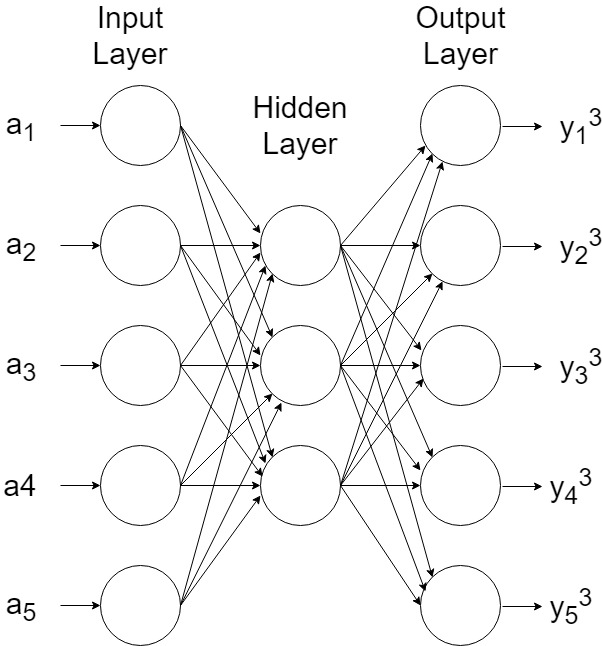
\includegraphics[width=0.5\columnwidth]{AE.jpg}
    \caption{Example of \ac{ae} architecture with $5$ input (and output) values and one hidden layer with 3 neurons.} 
    \label{fig:aeArch}
\end{figure}

For our \ac{irlv} problem, we train the \ac{ae} with attenuation vectors $\bm{a}^{(i)}$ taken only when the trusted \ac{ue} is in  \ac{roi} $\mathcal A_0$. Then, by letting $\bm{y}^{(L)}$ be the output vector of the \ac{ae} for the attenuation input $\bm{a}$, the \ac{mse} of the reconstruction is 
\begin{equation}\label{eq: rec err}
    \epsilon(\bm{a} ) = \frac{1}{N}\sum_{n=1}^{N}|a_n-y^{(L)}_n(\bm{a})|^2.
\end{equation}
Finally, the \ac{irlv} test function  is  
\begin{equation}
f(\bm{a}) =
\begin{cases}
1 &\text{if } \epsilon(\bm{a} ) \geq \Lambda, \\
-1 & \text{if } \epsilon(\bm{a} ) < \Lambda.
\end{cases}
\end{equation}

About the test power of the \ac{ae}, we observe that it can be seen as a quantization (or compression process) that quantizes an $N$-dimensional signal into an $M$-dimensional signal. In order to minimize the \ac{mse} of the reconstruction error, inputs with higher probability will have smaller quantization regions. Moreover, as the number of quantization points goes to infinity (since the quantization indices are in the continuous $M$-dimensional space) all points in the same quantization region will have approximately the same probability. However, quantization error for points within each region will be different for each point; in particular, equal to zero for the quantization point and greater than zero at the edges of the quantization region. Thus, we can conclude that the \ac{ae} can not provide as output the \ac{pdf} of the input even with infinite training and an infinite number of neurons, as required by the optimal decision rule (\ref{eq:oneClassDec}). On the other hand, input points with a smaller \ac{pdf} belong to larger quantization regions for which the reconstruction error is {\em on average} larger; therefore, the output provided by the \ac{ae} is on average monotonically decreasing with the \ac{pdf} of the input point. 

\begin{comment}
The performance of the obtained classifier are given by the following 
\begin{theorem}
    Consider a \ac{ae} with perfect training, i.e., a \ac{ae} with a sufficient number of neurons and a sufficient training. Then the classifier obtained by training the \ac{ae} and by thresholding the soft output $\tilde{\epsilon}(\bm{a}^{(n)}) = \sqrt{\frac{1}{N}\sum_{i=1}^{N}|a^{(n)}_i-\hat{a}^{(n)}_i|^2},$ is equivalent, in the \ac{mse} sense, to the optimal classifier \eqref{eq:oneClassDec}.
\end{theorem}
\begin{proof}
Let us consider the \ac{mse} approximation of $\tilde{\epsilon}(\bm{a}^{(n)})$ being $1/p(\bm{a}^{(n)}|\mathcal{H}_0)$ and hence consider the minimization problem over the weight vector $\bm{w}$
\begin{equation}
	\begin{aligned}
		&\underset{\bm{w}}{\text{min}}\,\, \Exp{ \left( \tilde{\epsilon}(\bm{a},\bm{w}) - \frac{1}{p(\bm{a}|\mathcal{H}_0)}\right) ^2} = \\
		&\underset{\bm{w}}{\text{min}} \int_{\bm{a} \in \mathbb{R}^n} \left[ \tilde{\epsilon}(\bm{a},\bm{w}) - \frac{1}{p(\bm{a}|\mathcal{H}_0)} \right] ^2 p(\bm{a}|\mathcal{H}_0) d\bm{a} = \\
		&\underset{\bm{w}}{\text{min}} \left\lbrace \int_{\bm{a} \in \mathbb{R}^n} \tilde{\epsilon}(\bm{a},\bm{w})^2 p(\bm{a}|\mathcal{H}_0) d\bm{a}
		-2\int_{\bm{a} \in \mathbb{R}^n} \tilde{\epsilon}(\bm{a},\bm{w}) d\bm{a}
		+ \int_{\bm{a} \in \mathbb{R}^n} \frac{1}{p(\bm{a}|\mathcal{H}_0)} d\bm{a} \right\rbrace.
	\end{aligned}	
\end{equation}
We notice that the second term in brackets is the sum of the reconstruction error of the attenuation vectors over $\mathbb{R}^{n}$. Since different regions of $\mathbb{R}^n$ are characterized by different features and since the \ac{ae} is able to reconstruct, with small reconstruction error, only those vectors with features similar to those of the training set we can assume that the summation of the reconstruction errors over all possible feature spaces goes to infinity. The second integral does not hence depend on $\bm{w}$ as for each value of $\bm{w}$ it goes to infinity. The last term in brackets does not depend on the weight vector $\bm{w}$ and hence the only term that depends on $\bm{w}$ is the first one, which is the objective function of the training optimization problem. Noticing that thresholding $\frac{1}{p(\bm{a}|\mathcal{H}_0)}$ with $\gamma$ is equivalent to thresholding $p(\bm{a}|\mathcal{H}_0)$ with $1/\gamma$ we conclude that training the \ac{ae} with $\epsilon$ loss function provides a classifier that approximates in the \ac{mse} sense the optimal one (\ref{eq:oneClassDec}).
\end{proof}
\end{comment}

\subsection{One-Class LS-SVM}

Similarly, we can resort to \ac{svm} to perform the one-class classification in \ac{irlv}. We focus in particular on the  \ac{oclssvm}, first introduced in \cite{choi2009least} as an extension of the one-class \ac{svm} \cite{Scholkopf2001estimating}. 

The only difference with respect to the \ac{svm} introduced in Section III is that the training optimization problem is now
\begin{subequations}
	\label{eq:oneClassSvm}
	\begin{equation}
	\label{eq:oneClass1}
	\underset{\bm{w},b}{\min} \quad \omega(\bm{w}, b) \triangleq
	 \frac{1}{2} \bm{w}^T \bm{w} +  \frac{C}{2} \sum_{i=1}^S e_i^2 +b
	\end{equation}
	\begin{equation}
	\label{eq:oneClassConstr}
	\text{subject to}\, -b - \bm{w}^T \phi (\bm{a}^{(i)})  = e_i,  \quad i = 1,\dots S, 
	\end{equation}
\end{subequations}
where $C$ is a hyper-parameter.
Note that in the one-class case, the bias parameter $b$ appears also in the objective function.


We observe also in this case that the one-class \ac{svm} is suboptimal, as it does not provides a monotone function of the \ac{pdf} of the input points. In fact, it is not necessary that the training points far from the bound of the classification region are less probable, and the direction $\bm{w}$ is obtained by an ensemble elaboration of the \ac{pdf} of the input rather then been a point-wise function of it (\hl{rileggere}). Nevertheless, by resorting to the Chernoff bound, we can conclude that by minimizing the \ac{mse} we also minimize the upper bound the probability of false alarm; therefore the optimization process goes in the right direction although not optimal.



\begin{comment}
We want to show that the \ac{oclssvm} is a machine that asymptotically approximate, in the mean-square sense, the optimal decision rule \eqref{eq:oneClassDec}.

\begin{lemma}
\label{lem:lem2}
Given $S$ training samples $\bm{a}^{(i)}$ from a finite alphabet $\mathcal C$, taken with a given static probability distribution, for large number of training samples, i.e., as $S \rightarrow \infty$, problem \eqref{eq:oneClassSvm} is equivalent to 
\begin{equation}
		\underset{\bm{w},e_i, \rho}{\text{min}} \Exp{e_i}^2
\end{equation}
\end{lemma}
\begin{proof}
We first proceed as in the proof of Theorem \ref{th:lsnp} and re-write problem \eqref{eq:oneClassSvm} as
	\begin{subequations}
		\label{eq:oclssvm22}
		\begin{equation}
		\label{eq:oclssvm2}
		\underset{\bm{w},e}{\text{min}} \quad f_0' = \frac{1}{2} \bm{w}^T \bm{w} + C S \frac{1}{2} \sum_{j=1}^M p_{\bm{a}^{(i)},t_i}(\bm{\alpha}_j,1) e_j^2 - \rho  
		\end{equation}
		\begin{equation}
		\label{eq:ocstpart2}
		\text{subject to}\,  \rho - \bm{w}^T \phi (\bm{a}^{(i)})  = e_i,  \quad i = 1,\dots M, 
		\end{equation}		
	\end{subequations} 
Note that differently from \eqref{eq:lssvm22} we have only $M$ constraints (and not $2M$) because we have target labels only of one class.
We now solve \eqref{eq:oclssvm22} using the same steps as in \cite{choi2009least}. Let us define the Lagrangian
\begin{equation}
	\mathcal{L} = 	\frac{1}{2} \bm{w}^T \bm{w} - \rho +
	C S \frac{1}{2} \sum_{j=1}^M p_{\bm{a}^{(i)},\hat{t}_i}(\bm{\alpha}_j,1) e_j^2 - 
	\sum_{j=1}^{M} u_j \left[ \bm{w}^T \phi (\bm{a}^{(j)}) -\rho + e_j \right],
\end{equation}
and set to zero the derivatives with respect to optimization variables and multipliers $u_j$

\begin{subequations}
\begin{equation}
\label{eq:derivatives1}
\frac{\partial \mathcal{L}}{\partial \bm{w}}: \quad \bm{w} = \sum_{j=1}^{M} u_j \phi (\bm{a}^{(j)}), 		
\end{equation}
  \begin{equation}
  \label{eq:derivatives2}
  		\frac{\partial \mathcal{L}}{\partial \bm{e_j}}: \quad CS p_{\bm{a}^{(i)},\hat{t}_i}(\bm{\alpha}_j,1) e_j = u_j \quad
  		 j=1,\dots, M,
  \end{equation}
  \begin{equation}
  \label{eq:derivatives3}
  		\frac{\partial \mathcal{L}}{\partial \rho}: \quad \sum_{j=1}^{M} u_j = 1
  \end{equation}
  \begin{equation}
  \label{eq:derivatives4}
  	\frac{\partial \mathcal{L}}{\partial \bm{u_j}}:	\quad \phi (\bm{a}^{(j)}) \bm{w} + e_j - \rho = 0.
  \end{equation}
\end{subequations}
Substituting \eqref{eq:derivatives1} and \eqref{eq:derivatives2} in \eqref{eq:derivatives4} we get the system of equations
\begin{equation}
\begin{aligned}
	&\sum_{i=1}^{M}  u_i k( \bm{a}^{(i)},\bm{a}^{(j)}) - \rho + \frac{u_j}{SCp_{\bm{a}^{(i)},\hat{t}_i}(\bm{\alpha}_j,1)}=0 \quad j = 1,\dots, M\\
	&\sum_{i=1}^{M}u_i=1,
\end{aligned}	
\end{equation}
with $M+1$ unknowns and $M+1$ equations which therefore provides finite convergence values for $\{\rho,u_i\}_{i=1}^{i=M}$. In the dual formulation of \eqref{eq:oneClassSvm} we can express $\bm{w}$ as a function of the kernel and Lagrange multipliers $\{u_j\}$ 
\begin{equation}
\bm{w}^T\bm{w} = \sum_{i=1}^{M} \sum_{j=1}^{M} u_i u_j k(\bm{\alpha}_i,\bm{\alpha}_j), 
\end{equation}
which, given the finiteness of the sum, converges.
We can now write
\begin{equation}
\begin{aligned}
\lim_{S \to +\infty} &\frac{1}{S} \bm{w}^T\bm{w} =0, \\
\lim_{S \to +\infty} &\frac{1}{S}\rho =0.
\end{aligned}		
\end{equation}
It follows that
\begin{equation}
	\underset{\bm{w},e_i, \rho}{\text{min}} \frac{1}{S} f_o(\bm{w},e_i, b) = 
	\underset{\bm{w},e_i, \rho}{\text{min}} \frac{1}{S} \sum_{i=1}^S e_i^2 = 
	\underset{\bm{w},e_i, \rho}{\text{min}} \Exp{e_i}^2,	
\end{equation}
where $e_i^2 = (\bm{w}^T \phi (\bm{a}^{(i)}) -\rho)^2 $, the last equality follows from the law of large numbers, and the expected value is carried out \wrt the training $\bm{a}^{(i)}$.
\end{proof}

%Note that $|e_i|$ is proportional, by a factor $1/||\bm{w}||$, to the distance between any point $\phi(\bm{a}^{(i)})$ and the hyperplane $\bm{w}^T \phi (\bm{a}) + b = 0$ defined in the transformed space by the \ac{oclssvm}. We claim that $|e_i|$ is inversely proportional to $p(\bm{a}|\mathcal{H}_0)$ and we will prove that this holds in the mean-square sense. A direct consequence is that the \ac{oclssvm} approximates asymptotically the optimal decision rule of Section \ref{sec:oneClassOpt}. 

\begin{theorem}
	\label{th:onelsnp}
	Consider a \ac{oclssvm} with perfect training, \ie the training reaches a global minimum of $f_o(\bm{w},e_i,b)$ given an infinite number of training points $\bm{a}^{(i)}$ drawn from the finite alphabet $\mathcal C$. Then the classifier obtained by training the \ac{oclssvm} and by thresholding the soft output \eqref{eq:svm} is equivalent, in the \ac{mse} sense, to the optimal classifier \eqref{eq:oneClassDec}.
\end{theorem}

\begin{proof}
Let $(\bm{w}^*,e_i^*, \rho^*)$ be the solution for problem \eqref{eq:oneClassSvm}. We note that $\rho^* >0$. If this was not the case, then we cold define the new triplet $(-\bm{w}^*,e_i^*, -\rho^*)$ providing a lower value for $f_o(\bm{w},e_i,\rho)$. This is because from \eqref{eq:oneClass1} the first two terms of the sum remain unchanged, while in the third term we are now subtracting a positive value, yielding
\begin{equation}
		f_o(-\bm{w}^*,e_i^*, -\rho^*) < f_o(\bm{w}^*,e_i^*, \rho^*).
\end{equation} 
Let us define the function 
\begin{equation}
	e(\bm{a},\bm{w},\rho) \triangleq \bm{w}^T  \phi (\bm{a}) - \rho,	
\end{equation}
and consider 
\begin{equation}
\label{eq:coreTheorem}
	\begin{aligned}
		&\underset{\bm{w},\rho}{\text{min}} \Exp{ \left( e(\bm{a},\bm{w},\rho) - \left(-\frac{1}{p(\bm{a}|\mathcal{H}_0)}\right)\right) ^2} = \\
		&\underset{\bm{w},\rho}{\text{min}} \int_{\mathbb{R}^n} \left[ e(\bm{a},\bm{w},b) + \frac{1}{p(\bm{a}|\mathcal{H}_0)} \right] ^2 p(\bm{a}|\mathcal{H}_0) d\bm{a} = \\
		&\underset{\bm{w},\rho}{\text{min}} \left\lbrace \int_{\mathbb{R}^n} e^2(\bm{a},\bm{w},\rho) p(\bm{a}|\mathcal{H}_0) d\bm{a}
		+2\int_{\mathbb{R}^n} e(\bm{a},\bm{w},\rho) d\bm{a}
		+ \int_{\mathbb{R}^n} \frac{1}{p(\bm{a}|\mathcal{H}_0)} d\bm{a} \right\rbrace.
	\end{aligned}	
\end{equation}
Consider the integral in the double product
\begin{equation}
		\int_{\mathbb{R}^n} e(\bm{a},\bm{w},b) d\bm{a} =
		\int_{\mathbb{R}^n} \bm{w} ^T  \phi (\bm{a})d\bm{a} - \int_{\mathbb{R}^n} \rho d\bm{a},		
\end{equation}
For what concerns the second integral in the r.h.s. we can write
\begin{equation}
		\int_{\mathbb{R}^n} \rho d\bm{a} = \rho \int_{\mathbb{R}^n} d\bm{a} = \sign(\rho) (+\infty) = + \infty,
\end{equation}
since we have shown that at the optimum $\rho^*>0$. Now, using \eqref{eq:derivatives1}, we can write the first integral as
\begin{equation}
\begin{aligned}
		&\int_{\mathbb{R}^n} e(\bm{a},\bm{w},\rho) d\bm{a} = \int_{\mathbb{R}^n} \sum_{j=1}^{M} u_j k(\bm{a}^{(j)},\bm{a})d\bm{a} \\
		&= \sum_{j=1}^{M} u_j \int_{\mathbb{R}^n} k(\bm{a}^{(j)},\bm{a})d\bm{a} = \int_{\mathbb{R}^n} k(\bm{a}^{(j)},\bm{a})d\bm{a},
\end{aligned},
\end{equation}
where we used \eqref{eq:derivatives3}.
Note that the only term in the last line of \eqref{eq:coreTheorem} that depends on the optimization variables $\{\bm{w}, \rho \}$  is 
\begin{equation}
		\Exp{  e^2(\bm{a}, \bm{w}, \rho)} = \int_{\mathbb{R}^n} e^2(\bm{a},\bm{w},\rho) p(\bm{a}|\mathcal{H}_0) d\bm{a},
\end{equation}
which, from Lemma \ref{lem:lem2} is, asymptotically, the objective function optimized by the \ac{lssvm}.
%The third term inside the curly brackets does not depend on $(\bm{w},b)$. Therefore, the mean square error approximation of $1/p(\bm{a}|\mathcal{H}_0)$ is found by minimizing $\Exp{e^2(\bm{a},\bm{w},b)}$ which, by Lemma \ref{lem:lem2}, is the same function minimized by \ac{oclssvm}. Asymptotically we have, from \eqref{eq:svm},
%\begin{equation}
%\label{eq:approx}
%	\tilde{t} \approx \frac{1}{p(\bm{a}|\mathcal{H}_0)},	
%\end{equation} 
%in the mean square sense. Note that thresholding $\frac{1}{p(\bm{a}|\mathcal{H}_0)}$ with $\gamma$ is the same as thresholding $p(\bm{a}|\mathcal{H}_0)$ with $1/\gamma$ which is the optimal classifier of Section \ref{sec:oneClassOpt}.
\end{proof}
\end{comment}

\subsection{\ac{ml}-Based Attack Strategies}
\label{sec:attack}
\hl{LA TOGLIAMO??}

\revi{sezattack}{Until now we have used ML approaches to perform \ac{irlv}. Here we propose to use ML also to obtain new more powerful attacks. In particular, we focus on an attacker that moves outside $\mathcal A_0$ and performs multiple attacks. We assume that the attacker knows if each attack is successful or not, and aims at minimizing the number of attacks before success. Moreover, we assume that before attack the attacker can estimate the attenuation vector to each \ac{ap}, by exploiting training signals transmitted by the \acp{ap}: while these estimate come almost for free to the attacker, an active attack is more expensive, both in terms of transmitted energy and as an intense attack sequence can be detected by the \acp{ap} that can take suitable countermeasures, which however are outside the scope of this work. Therefore we simply focus on the problem of doing as few attacks are possible, while being able to have as much attenuation vectors of the area outside $\mathcal A_0$. The proposed strategy works as follows:}
\begin{enumerate}
    \item The attacker visit  $N$  points spread uniformly at random outside $\mathcal A_0$. From each point it collects the attenuation vector and performs the attack. If any of the attacks is successful, the procedure is stopped.
    \item If none of the $N$ attacks has been successful, the attenuation vectors are used to train a one-class classifier.
    \item The attacker picks a new position uniformly at random outside $\mathcal A_0$ and feeds its attenuation vector to the trained classifier.
    \item If the vector is classified as belonging to the class it is discarded, and the procedure goes back to point 3), otherwise an attack from that position is performed.
    \item If the attack is successful, the procedure is stopped. Otherwise, the attenuation vector is used to as further training input of the one-class classifier and the procedure goes back to point 3).
\end{enumerate}
\revi{sezattack2}{Note that other attack strategies are possible, including game-theoretic approaches, where the attacker and the \ac{irlv} system are confronting players. These strategies are left for future study and we concentrate on the described attack procedure as it is similar, while from the attack perspective, to that used by the \ac{irlv}.}

\begin{comment}
\ac{ml} techniques can be also exploited in order to perform more effective attacks. In particular, the attacker can $a$) compute estimates of the attenuation vectors of its channel to all the \acp{ap}, and $b$) move around in the area $\mathcal A_1$ and perform attacks. Point $a$) is possible if \acp{ap} transmit training signals to the \ac{ue}, so that it can estimate the channel characteristics. We also assume that the attacker has means to determine if its attack has been successful, e.g., by receiving the services reserved to \acp{ue} in the \ac{roi}.

%Consider a training set set large enough to cover the statistical description of the non-legitimate area $\mathcal{A}_1$. The attenuation vector with the highest reconstruction error in the \ac{ae} case or with the largest value of $\tilde{t}_o$ in the \ac{oclssvm} case can be considered at the border of the region $\mathcal{A}_1$, and hence nearer to region $\mathcal{A}_0$. In the next section we describe two attack strategies exploiting this property of the \ac{ml} algorithms: the former attack is the filter attack, which exploits the one class trained \ac{ml} algorithms to select proper attack vectors; the latter is the gradient based attack, which exploits the loss function of \ac{ml} algorithms in order to forge attenuation vectors that can be considered as authentic by the \ac{irlv} system.

%\subsection{Selective \ac{ml} Attack}


%Although it is possible to perform multiple attacks, 
The purpose of the attacker is to be successful with the minimum number of attacks in order not to let the network detect to be under a series of attacks and take countermeasures (e.g., activating additional \ac{irlv} techniques or switching off the service). Moreover, a smaller number of attacks reduces the resource consumption by the attacker and provides faster access to the services. In order to make attacks more efficient, we propose that the attacker 1) moves in the \ac{roi}-complementary area $\mathcal A_1$, 2) measures the attenuation vectors at various position, and then 3) decides whether to attack or not according to its previous experience of failed attacks. We denote this attack as {\em selective \ac{ml} attack}. As soon as an attack is successful, the procedure is stopped; therefore, the data on which the attacker can use to take his decision comprises only failed attacks.

In details, the attacker uses the attenuation vectors of (failed) attacks to train a one-class classifier. Then, when reaching a new position it feeds the attenuation vector to the classifier and, if it is classified as belonging to the same class of training, no attacks is performed since the position is deemed to be useless. Otherwise, if the attenuation vector is not recognized as belonging to the class of collected points, it is evaluated as a potential successful attack and the attacker sends a message claiming to be in $\mathcal A_0$ to the network. If successful, the procedure is stopped, while upon failure the attenuation vector is fed as additional training data to the machine so that the classifier becomes more accurate.  
\end{comment}
%As before stated the one class classification involves training the \ac{ml} algorithms with attenuation vectors measured from one of the two available classes. We here propose an attack strategy which trains the \ac{ml} algorithms with attenuation vectors measured from the non-legitimate area $\mathcal{A}_1$. However, differently from a simple random attack, the attenuation vectors are \emph{filtered} by the attacker with a machine trained to learn the class of non successful points. The chosen attack point is then only the one yielding the worst metric as output of the filter. In this way we aim at minimizing the number of attempted attacks.

%In particular, consider an attenuation vector $\bm{a}_{\mathcal{A}_1}$ measured in area $\mathcal{A}_1$ This vector could be a possible successful attack and is hence tested. If the attack is not successful $\bm{a}_{\mathcal{A}_1}$ is used to train the \ac{ml} algorithm. 
%We generate $n_{\rm x}$ spatial coordinates located in area $\mathcal{A}_1$ and we measure the attenuation values incurred in each position. We then filter this set of vectors with the \ac{ml} algorithm and select as a possible attack the vector which is more likely to belong to class $\mathcal{A}_0$ (i.e., the one with highest reconstruction error for the \ac{ae} and with smallest $\tilde{t}_0$ for the \ac{oclssvm}). If the selected vector is not a successful attack then it is used to update the training of the \ac{ml} algorithm.

For the one-class classifier, we use either the \ac{ae} or the \ac{svm}, as described in the previous section. 
%
% This process is repeated until a successful attack vector is generated. The algorithm steps are shown in Algorithm \ref{alg:filter}.
%
%\begin{algorithm}[t]
%\label{alg:filter}
%  \algsetup{linenosize=\tiny}
%  \scriptsize
%
% \KwData{ $\bm{a}_{\mathcal{A}_1}$}
% \KwResult{successful attack vector }
% 
%
% \Repeat{attack is successful}{
%        \eIf{first attack}{
%        test $\bm{a}_{\mathcal{A}_1}$\;
%        \If{attack $\neq$ successful}{
%        build and train the \ac{ml} architecture with $\bm{a}_{\mathcal{A}_1}$\;
%        }
%        }
%        {
%        build set $\bm{A}$ of randomly selected attenuation vectors from $\mathcal{A}_1$\;
%        $\bm{a}_{\mathcal{A}_1} = \underset{\bm{a} \in \bm{A}}{\max} \quad \rm{loss} \, \rm{function}$ $(\bm{A})$\;
%        \If{attack $\neq$ successful}{
%       update training with $\bm{a}_{\mathcal{A}_1}$
%       }
%      }
%      }
%    
% \caption{Selective \ac{ml} attack}
%\end{algorithm}

%Note that Point $b$) is possible by letting the attacker to be equipped with multiple antennas so that, thanks to the estimates its channel to the \acp{ap}, the attacker can beamform the training signals with different gains to the \acp{ap}, thus letting them estimate the intended attenuation values. In this setting even a static \ac{ue} can generate many attacks with different estimated attenuation vectors at the \acp{ap}. 

% \subsection{Gradient-based \ac{ae} attack}
% Consider the set $\bm{A}$ of the attenuation vectors from $\mathcal{A}_1$ used for training the attacker \ac{ae}. The vector with highest reconstruction error is selected as a starting point for a possible successful attack. In order to find a direction toward which move the values of the attenuation vector to increment the probability of a successful attack, knowing that a higher reconstruction error means an higher probability of the vector belonging to the authentic area $\mathcal{A}_0$, we perform a gradient ascent algorithm based on the reconstruction error function (\ref{eq: rec err}) . 
% Starting from the attenuation vector with highest reconstruction error we perform various steps of the gradient algorithm and, for each step we exploit the forged vector as a possible attack. Considering the first attack as $\bm{a}_f^{(0)}=\underset{\bm{a} \in \bm{A}}{\max}$ the attack vector at iteration $q$ is
% \begin{equation}\label{eq: rnn attack}
%     \bm{a}_f^{(q)} = \bm{a}_f^{(q-1)}+ \delta \nabla_{\bm{a}}\epsilon(\bm{a}_f^{(q-1)}).
% \end{equation}
% The gradient ascent algorithm continues up to the point where the attack is successful or when the reconstruction error is lower then the one obtained in the previous step, i.e., $\epsilon(\bm{a}_f^{(q)}) < \bm{a}_f^{(q-1)}$. When the algorithm stops due to the second case the training of the \ac{ae} is updated with $\bm{a}_f^{(q-1)}$. The new training set is hence updated as $\bm{A} = \bm{A} \cup \bm{a}_f^{(q)}$ and the attenuation vector with highest reconstruction error obtained by the updated \ac{ae} is selected as the new starting point of the gradient algorithm. The algorithm steps are shown in Algorithm \ref{alg:rnnGrad}.

% \begin{algorithm}[t]
% \label{alg:rnnGrad}
%   \algsetup{linenosize=\tiny}
%   \scriptsize

%  \KwData{ trained \ac{ae}, training set $\bm{A}$, $\delta$}
%  \KwResult{successful attack vector }
 

%  \Repeat{attack is successful}{
%         select $\bm{a}_f^{(0)} = \underset{\bm{a} \in \bm{A}}{\max}\epsilon(\bm{a})$ \;
%         test $\bm{a}_f^{(0)}$ as attack \;
%         \If{$a_f^{(0)}$ is not successful}{
%         \Repeat{attack is successful or $\epsilon(\bm{a}_f^{(q)}) < \bm{a}_f^{(q-1)}$}
%         {
%         generate attack $\bm{a}_f^{(q)}$ via (\ref{eq: rnn attack})\;
%         perform the attack \;
    
%       }
%       \If{attack is not successful $\&$ $\epsilon(\bm{a}_f^{(q)}) < \bm{a}_f^{(q-1)}$}
%         	{$\bm{A}=\{\bm{A},\bm{a}_f^{(q)}\}$\;
%             update training of the \ac{ae} \;}
%             }
%       }
    
%  \caption{Gradient-based \ac{ae} attack}
% \end{algorithm}


% \subsection{\Acl{oclssvm} Attack}
% The attacker trains a \ac{oclssvm} with the training data coming only from the non-authentic area and his objective is now to forge an attack value $\bm{a_{f}}$ that will be accepted as authentic by the \ac{irlv} system. We propose an euristic approach  exploiting the fact that the test function for the attacker's trained \ac{oclssvm} would be
% \begin{equation}
% \bm{a} \in
% 	\begin{cases}
% 		\mathcal{A}_1 \quad \text{if} \quad \tilde{t} \geq \Lambda \\
% 		\mathcal{A}_0 \quad \text{if} \quad \tilde{t} < \Lambda.
% 	\end{cases}	
% \end{equation} 
% Moreover, from Theorem \ref{th:onelsnp} we know that the more $\tilde{t}$ decreases, the more $p(\bm{a}|\mathcal{H}_0)$ decreases as well.
% This suggests that the attacker could start from the training point $\bm{a}_{f}^{(0)}$ yielding the lowest value of $\tilde{t}$ and then moving along the direction of greatest decrease $\bm{d}$, given by
% \begin{equation}
% \label{eq:dDef}
% 	\bm{d} \triangleq - \nabla_{\bm{a}} \tilde{t},
% \end{equation} 
% where $\nabla_{\bm{a}}$ is the gradient operator \wrt $\bm{a}$. Exploiting the dual formulation \cite{choi2009least} we can write
% \begin{equation}
% \label{eq:gradient}
% 		\nabla_{\bm{a}} \tilde{t} = \sum_{j=1}^{S} u_j \nabla_{\bm{a}} k(\bm{a}_j,\bm{a}).
% \end{equation}
% Using the radial-basis kernel
% \begin{equation}
% k(\bm{a}_j,\bm{a}_i) = e^{-\frac{||\bm{a}_j-\bm{a}_i||^2}{2\sigma^2}},
% \end{equation}
% the explicit expression for the gradient in \eqref{eq:gradient} is
% \begin{equation}
% 	\nabla_{\bm{a}} \tilde{t} =\frac{1}{\sigma^2} \sum_{j=1}^{S} u_j k(\bm{a}_j,\bm{a}) (\bm{a}_j - \bm{a}).
% \end{equation}
% Next, the attacker forges the point
% \begin{equation}
% 	\bm{a}_f^{(1)} = \bm{a}_f^{(0)} + \delta \bm{d}, 	
% \end{equation}
% where $\delta$ is a parameter, and performs the attack. If it does not succeed, he re-trains the \ac{oclssvm} with this new information and repeats the attack until he eventually succeeds. This constitutes Algorithm \ref{alg:svm}.

% \begin{algorithm}[t]
% \label{alg:svm}
%   \algsetup{linenosize=\tiny}
%   \scriptsize

%  \KwData{ Training set, $\delta$}
%  \KwResult{succesful attack vector }
 

%  \Repeat{attack is succesful}{
%  		train a \ac{oclssvm} \;
%         select $\bm{a}_{f}^{(0)}$ yielding the lowest value of $\tilde{t}$ \;
%         compute $\bm{d}$ from \eqref{eq:dDef} \;
%         compute $\bm{a}_f^{(1)} = \bm{a}_f^{(0)} + \delta \bm{d}$ \;
%         perform the attack \;
%         \If{
%         	attack is not succesful}
%         	{$\bm{a}_f^{(1)}$ belongs to non-authentic area\;
%         	add $\bm{a}_f^{(1)}$ to training set\;}
%       }
    
%  \caption{One-class \ac{svm} Attack}
% \end{algorithm}


\section{Numerical Results}\label{sec:numRes}


In this section, we present the numerical results obtained using the proposed \ac{irlv} and attack solutions for the scenario described in Section II. (\hl{Qui inserirei un breve riassunto dell'experimental setup, non solo per le NN. Giorgio}) \revi{activation}{In particular, for the \ac{nn} for two-class classification, the activation function for the input layer is the identity function and for the hidden layer is the sigmoid function}
\begin{equation}\label{eq:sigmoid}
\psi^{(1)}(x) = \frac{1}{1-e^{-x}},
\end{equation}
\revi{activation2}{For the output layer the choice of the output function depends on the used loss function. Considering the \ac{ce} based \ac{mlp} tho problem we aim at solving is classification. As the output of the \ac{mlp} should be $0$ for \acp{ue} located in $\mathcal{A}_1$ and $1$ for \acp{ue} located in $\mathcal{A}_0$, the output function should be continuous in the interval $[0,1]$. An usual choice for the activation function for} \hl{Ruvoletto}
\begin{equation}
\psi^{(1)}(x)=\tanh^{-1}(x) = \frac{1}{2} \left( \frac{1+x}{1-x} \right).
\end{equation}
In order to build the training set, we consider $n_x$ spatial points $\bm{x}_{\rm UE}$, each one representing the coordinates of the position of a \ac{ue}, uniformly distributed over the area $\mathcal A$.

About the channel model, we consider a unitary transmitting power for each user and a carrier frequency of $f_0=2.12$ GHz. The path-loss coefficient is $\nu=3$, the shadowing power is \revi{shadVar}{$\sigma_s^2=8$ dB} and the shadowing decorrelation distance is $d_c=75$ m. 


\subsection{Two-class \ac{irlv} With Single \ac{ap}}\label{sec:singleAp}

We consider here the \ac{irlv} system using a single \ac{ap}. Two channel models are considered: a simple \ac{los} channel model as discussed in Section \ref{sec:los}, and a no-\ac{los} model including both path-loss and shadowing.

\paragraph*{\ac{los} Model} \revi{numResSimplScen}{We consider the simplified scenario of Section \ref{sec:los} with $R_{\rm out}= 10$ meters, $R_{\rm in} = 2$ meters and $R_{\rm min} = 0.1$ meters. We here compare the performance of the system for the two different scenarios, i.e., the fading scenario and the shadowing scenario, with the machine learning approaches. In particular, for the fading scenario we consider the cases $\nu=2$ and $\nu=3$ where the \ac{llr} functions used for the \ac{np} test are given by (\ref{eq:llr1}) and (\ref{eq:llr2}), whereas for the shadowing scenario we consider $\nu=2$ and $\sigma_s^2 = \{-8,0,0\}$ dB and the \ac{llr} for the \ac{np} framework is given by (\ref{eq:llr3}). For the \ac{ml} approaches, we consider $S=10^5$ training points and $N_L = 2$ hidden layers each with $N_h=5$ neurons.}

\begin{figure}[h]
    \centering
    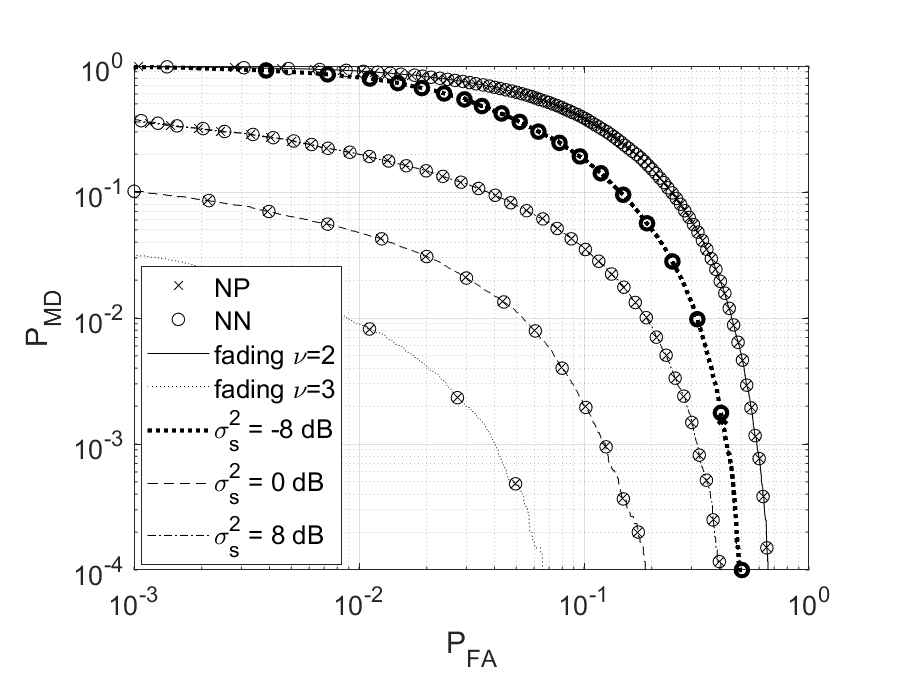
\includegraphics[width=0.6\columnwidth]{comp_NN_NP_CE.eps}
    \caption{\ac{roc} of \acp{irlv} methods in the scenarios of Section \ref{sec:los}: comparison between \ac{np} framework and \ac{nn}.}
    \label{fig:ceVSnp}
\end{figure}

\begin{figure}[h]
    \centering
    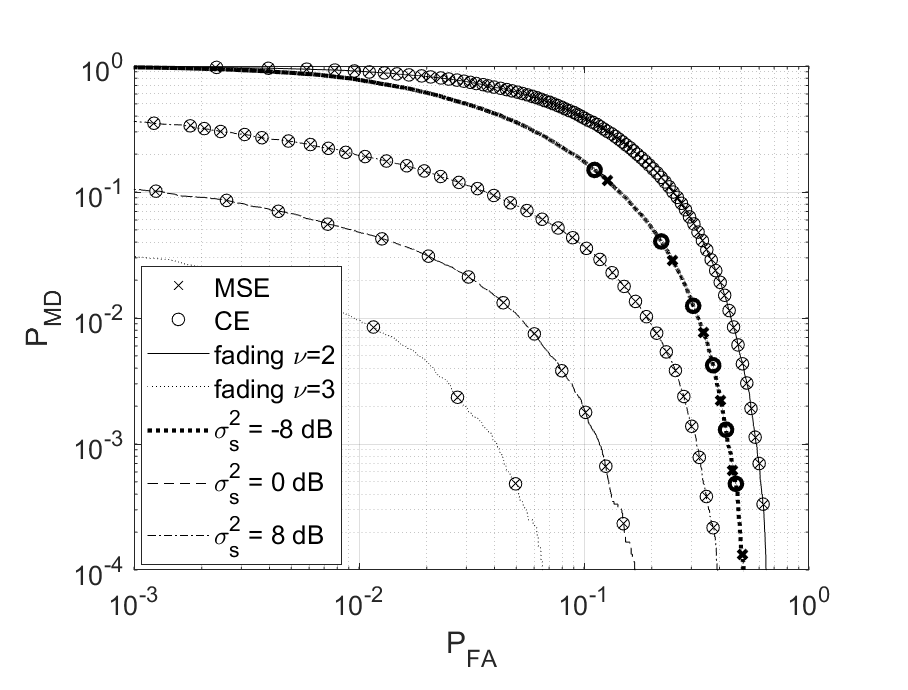
\includegraphics[width=0.6\columnwidth]{comp_NN_CE_MSE.eps}
    \caption{\ac{roc} of \acp{irlv} methods in the scenarios of Section \ref{sec:los}: comparison between \ac{ce} and \ac{mse} trained \acp{nn}. $S=10^5$ training points and $N_L = 2$ hidden layers each with $N_h=5$ neurons}
    \label{fig:ceVSmse}
\end{figure}

\revi{numResSimplScen2}{Fig. \ref{fig:ceVSnp} shows the \ac{fa} versus (vs.) the \ac{md} probabilities -- the so-called \ac{roc} --  obtained with two \ac{irlv} techniques: the \ac{np} test functions for the different scenarios and the \ac{mlp} designed with \ac{ce} loss function. We notice that the performance of the \ac{mlp} based system achieve the same values obtained with the \ac{np} framework. This numerical results confirm that hypothesis testing implemented via \ac{mlp} is optimal in the \ac{np} sense.}

\revi{numResSimplScen3}{Fig. \ref{fig:ceVSmse} shows the \ac{fa} vs. the \ac{md} probabilities comparing \ac{mlp} with \ac{ce} and \ac{mse} loss functions. We note that both \ac{nn}-\ac{ce} and \ac{nn}-\ac{mse} obtain the same performance for the same number of layers $N_L$ and neurons $N_h$ per layer as expected, since they both are equivalent to \ac{np} testing in the asymptotic regime.}

\revi{numResSimplScen4}{In general we notice that fading has a deeper impact on the system performance. However by increasing the value of the path loss coefficient $\nu$ we achieve better results, as the exponential random variable representing the received power has a smaller tail and hence hypothesis testing has lower uncertainty. Non correlated shadowing has better performance than the fading case as the received power is, in the logarithmic domain, affected by the sum of path loss and a Gaussian random variable. Hence, the smaller the variance $\sigma_s^2$, the smaller the uncertainty on the path loss, and hence the higher the performance of the \ac{irlv} system.}

\paragraph*{No-LOS Scenario} 

\begin{figure}[t]
    \centering
    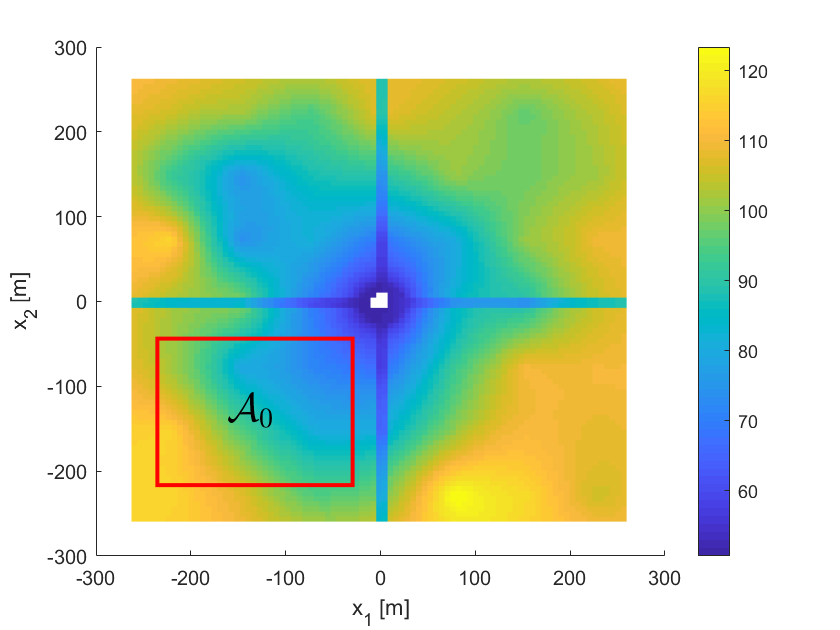
\includegraphics[width=0.6\columnwidth]{surfColorato.png}
    \caption{Example of attenuation map including path-loss and shadowing in the non-\ac{los} scenario.}
    \label{fig:map}
\end{figure}

We now consider a more general channel model including shadowing and no-\ac{los} and more general shapes of $\mathcal A$ and $\mathcal A_0$. With reference to Fig. \ref{fig:map} we focus on a scenario in which the \ac{ap} is located at the center of the map. Moreover, we have a Manhattan grid with two streets crossing at the center of a square region. \revi{building}{We consider as the \ac{roi} a space located inside the building located in the south-west corner of the map. A scenario of this type can model a situation where access to network services is granted only to users located inside an office.} Along the streets, \ac{los} propagation conditions are present, while no-\ac{los} propagation conditions are present in the rest of the area. Fig. \ref{fig:map} shows a realization of the  attenuation map including path-loss and shadowing. We can see \ac{los} propagation conditions along the streets and no-\ac{los} propagation conditions in buildings.

Also in this scenario, we do not expect to be able to achieve simultaneously low \ac{md} and \ac{fa} probabilities by using a single \ac{ap} ($N_{\rm AP} =1)$. Indeed, when compared to the \ac{los} scenario, the presence of shadowing increases the ambiguity on the attenuation inside and outside the region. However, we can compare \ac{ml} and \ac{np} \ac{irlv} approaches.  

%Consider the \ac{llr} (\ref{eq:lr}). In the no-\ac{los} context the computation of the two area dependent probabilities has no closed-form solution. A numerical solution is obtained by sampling the attenuation values over the spatial grid of positions and computing the area dependent distributions of the attenuation values. Consider an attenuation value $\hat{a}$: the probability of measuring $\hat{a}$ given that the \ac{ue} is located in area $\mathcal{A}_0$ is given by the number of positions $(x_u,y_u) \in \mathcal{A}_0$ where the measured attenuation $a(x_u,y_u)=\hat{a}$ over the total number of positions $(x_u,y_u)$ in the entire map having the same attenuation $\hat{a}$, i.e.
%\begin{equation}
%    \mathbb{P}(\hat{a}|\mathcal{A}_0) \approx \frac{\text{number of positions} \, (x_u,y_u) \in \mathcal{A}_0 \, \text{s.t.} \, a(x_u,y_u) = \hat{a}}{\text{total number of positions} \, (x_u,y_u) \, \text{s.t.} \, a(x_u,y_u) = \hat{a}}
%\end{equation}
%With the same reasoning we compute $\mathbb{P}(\hat{a}|\mathcal{A}_1)$, and an approximation of equation (\ref{eq:lr} is hence obtained as
%\begin{equation}\label{eq:lrApp}
%    \mathcal{L} \approx \frac{\text{number of positions} \, (x_u,y_u) \in \mathcal{A}_0 \, \text{s.t.} \, a(x_u,y_u) = \hat{a}}{\text{number of positions} \, (x_u,y_u) \in \mathcal{A}_1 \, \text{s.t.} \, a(x_u,y_u) = \hat{a}}
%\end{equation}
%The value computed by (\ref{eq:lrApp}) gets closer to the real value as the number of grid points over the map increases, as an higher number of points means a better statistical characterization of the attenuation over the map area.

Since no close-form expression of the \ac{llr} is available in this case, we start from the collected data in the learning phase, then, we quantize the attenuation values with a large alphabet and estimate the sampled \ac{pdf} for the quantized attenuation to be used in the \ac{llr} computation. For the considered scenario with path-loss and shadowing, we use $4.46 \cdot 10^6$ training points in the area and a uniform quantizer for the attenuation was considered with $300$ quantization values. On the other hand, we use only $10^3$ points for training both \ac{mlp} and \ac{svm}. 

Fig. \ref{fig:trueMap} shows the \ac{roc}  of \ac{np}, \ac{nn}-\ac{ce} and \ac{ls}-\ac{svm} obtained by averaging over many attenuation maps with different shadowing (\hl{how many? giorgio}). The \ac{np} test function has been obtained from the sampled \ac{pdf}, as just described. We notice that both \ac{nn}-\ac{ce} and \ac{ls}-\ac{svm} outperform the \ac{np} test. This means that even for very large numbers of samples available to estimate the \ac{pdf}, we still we have a performance degradation with respect to perfect knowledge of the statistics which would outperform all other methods. On the other hand, a relatively smaller number of training points for \ac{ml} methods already provide more powerful test functions showing the effectiveness of \ac{ml} techniques when no channel statistics is available a-priori. Therefore, in the following sections we drop the \ac{np} method and we consider large training datasets and more layers/neurons for the \ac{nn} in order to achieve close-to-optimal performance.
 
\begin{figure}[t]
    \centering
    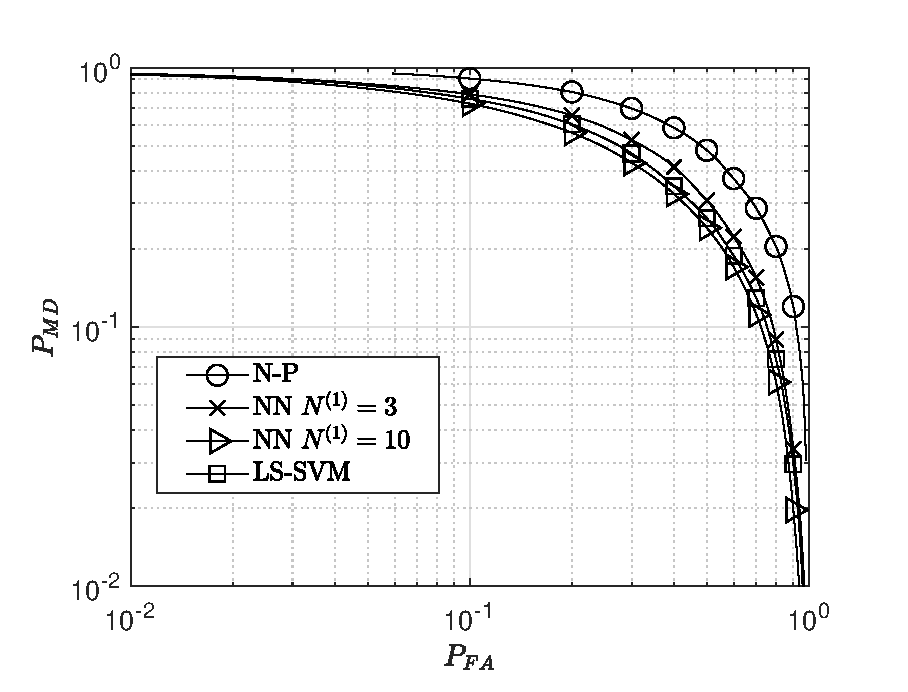
\includegraphics[width=0.6\columnwidth]{res_NP_approx_SVM.eps}
    \caption{\ac{roc} for a scenario with path-loss and shadowing for \ac{np}, \ac{svm} and \ac{mse}-\ac{nn} and hidden layer $N_h$ neurons.}
    \label{fig:trueMap}
\end{figure}

%Comparing the number of grid points and the number of training points used for the \ac{ml} algorithms we can conclude that the \ac{ml}-based solution is advantageous over the \ac{np}-based one, as it requires a smaller number of points in order to get an estimate of the area dependent probabilities. Furthermore this implies that the \ac{ml}-based \ac{irlv} system can be implemented without any a-priory knowledge of the \ac{pdf} of the hypothesis to be tested.

\subsection{Two-class \ac{irlv} With Multiple \acp{ap}}
\label{sec:res_fading}

\begin{figure}[t]
    \centering
    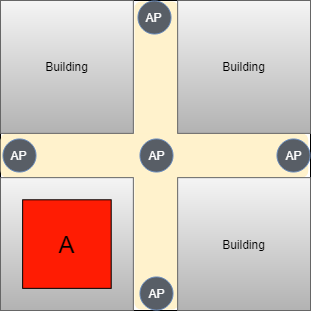
\includegraphics[width=0.5\columnwidth]{scenario2.png}
    \caption{Scenario with $N_{\rm A} =5$ \acp{ap}, the side of the square representing area $\mathcal A$ has a length of 525 m, while the side of area $\mathcal A_0$ has a length of 255 m.} 
    \label{fig:mBS}
\end{figure}
\begin{figure}[t]
    \centering
    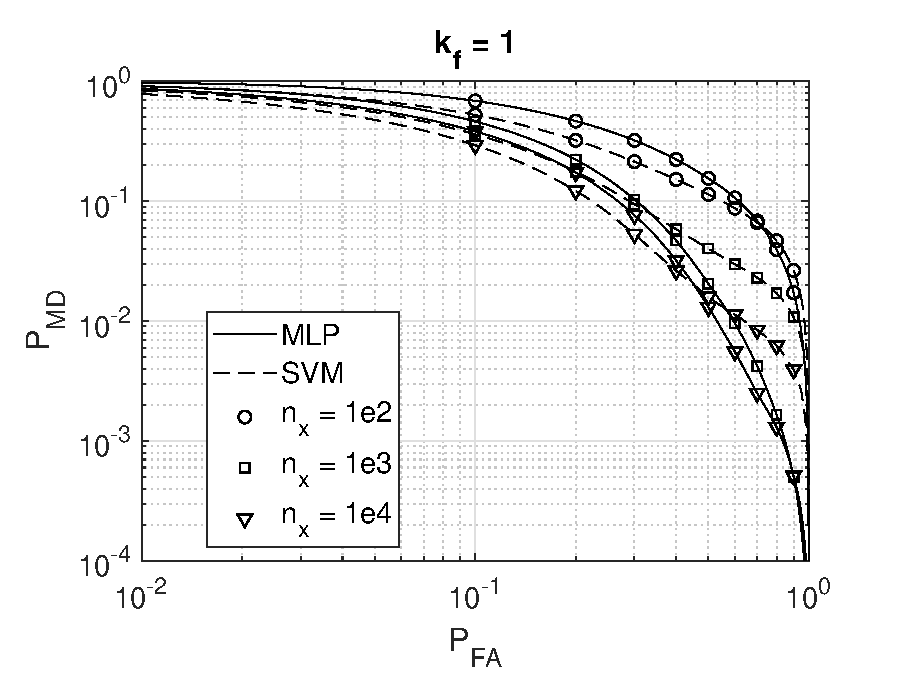
\includegraphics[width=0.6\columnwidth]{res_avg_nTrain_kf1.eps}
    \caption{\ac{roc} of \ac{svm} and \ac{nn}-\ac{ce} ($N_h = 10$) for different numbers of training set size $S$.}
    \label{fig:kf1}
\end{figure}

In Fig. \ref{fig:mBS}, we consider a network with $N_{\rm ap}=5$ \acp{ap} used for \ac{irlv} and a square area $\mathcal A$ with side length of 525 meters, while the \ac{roi} $\mathcal A_0$ is a square with side length of 255 meters. 
We include also fading into the channel model, as introduced in Section II.

Fig. \ref{fig:kf1} shows the \ac{roc} for \ac{nn}-\ac{ce}  (with $N_h = 10$) and \ac{ls}-\ac{svm} \ac{irlv} methods and different values of the training set size $S$. We observe that for the same  \ac{fa} probability  we achieve a lower \ac{md} probability as the size of the set $S$ increases, and that both methods performs in a similar way with large a training set, as we know that they both converge to the optimal \ac{np} solution, not reported here for the difficulty of obtaining the \ac{llr}, as discussed above (\hl{rileggere ultima frase}). Moreover, with multiple \acp{ap}, we can better distinguish attenuation vectors associated to \ac{ue} positions inside and outside the \ac{roi} with respect to the scenario with a single \ac{ap}. Still, for security purposes, we would prefer even lower values of \ac{fa} and \ac{md} probabilities; this can be achieved, for example, by increasing the number of \acp{ap} or considering other channel features, e.g., its wideband impulse response. 


\begin{figure}[t]
    \centering
    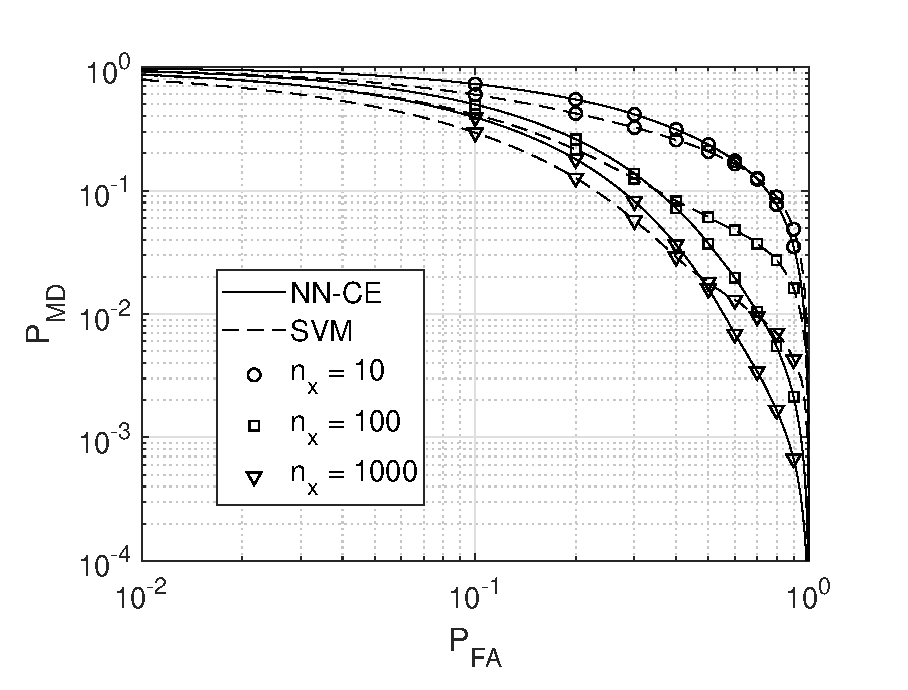
\includegraphics[width=0.6\columnwidth]{res_avg_nTrain_kf10.eps}
    \caption{\ac{roc} of \ac{svm} and \ac{nn}-\ac{ce} ($N_h = 10$) for different numbers of collected locations ($n_x$) and $k_f=10$ fading realization per location.}
    \label{fig:kf10}
\end{figure}

(\hl{forse squi una sottosezione. giorgio}) We now investigate the choice of the points used for training of the \ac{ml} approaches in the presence of fading. First, note that for a given \ac{ue} position, the attenuation takes various values over time according to the instantaneous fading realization. Therefore, we want to study whether the collection of multiple attenuation vectors for each explored location in the training phase has an impact on the performance of the classifier.  Let $n_x$ be the number of explored locations by the \ac{ue}, and $k_f$ the number of collected fading realizations per location. Overall, we obtain $S = n_x \cdot k_f$ training attenuation vectors. For example, Fig. \ref{fig:kf1} is obtained with $k_f=1$ as each training point is associated to a different uniform randomly generated location. Fig. \ref{fig:kf10} instead shows the \ac{roc} for the same values of $S$ of Fig. \ref{fig:kf1}, but with $k_f=10$ fading realizations per location (thus $n_x = S/10$). By comparing the two figures, we note that for small values of $S$, the performance get slightly worse as $k_f$ grows. For a large enough training set size $S$, different values $k_f$ provide approximately the same performance.  Therefore, we can conclude that, for large training sets, \ac{ml} algorithms are also robust to fading irrespective of the number of collected fading realization per location. However, in practical situations where the points for training may be limited, it may be advantageous to collect more fading realization per location. 


\subsection{One-Class \ac{irlv} With Multiple \acp{ap}}\label{sec:numResOneClass}

\begin{figure}[t]
    \centering
    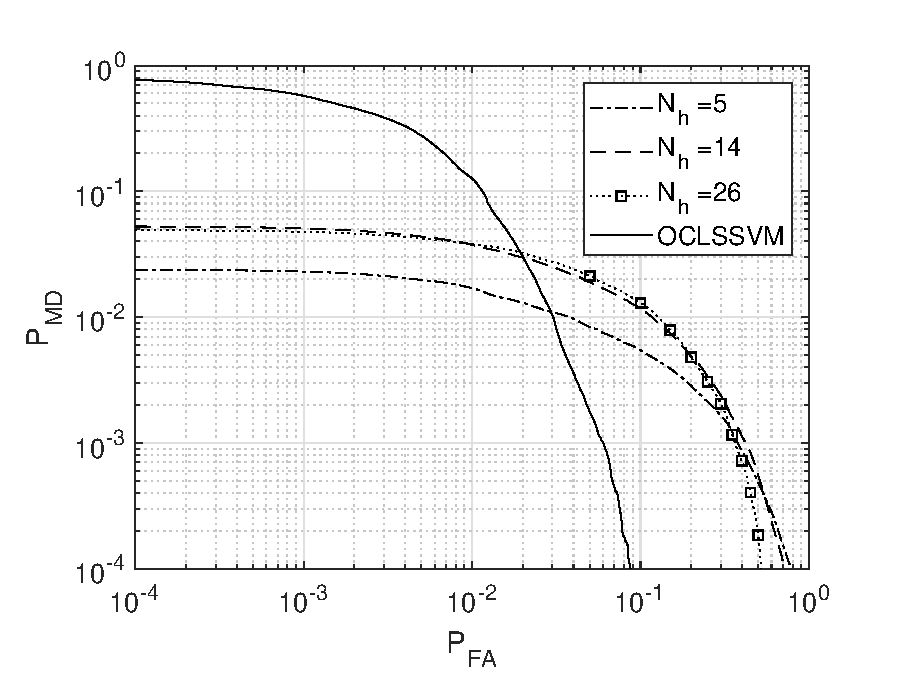
\includegraphics[width=0.6\columnwidth]{res_ae_onNeur.eps}
    \caption{\ac{roc} for one-class \acp{irlv} in a scenario with path-loss, shadowing and without fading.}
    \label{fig:aeNh}
\end{figure}

We now focus on the one-class \ac{irlv} solutions, where the training points come only from the \ac{roi} $\mathcal A_0$. \revi{designAE}{The \ac{ae} has been implemented by considering the activation functions in \cite{Hinton-2006}. All neurons use logistic sigmoid activation function (\ref{eq:sigmoid}) except for the central hidden layer which is linear.} We first consider a scenario with path-loss and shadowing without fading.

Fig. \ref{fig:aeNh} shows the \ac{roc} for both \ac{oclssvm} and \ac{ae} with $N_h \in [1, 5]$ and $S=10^4$ training vectors. We see that, by increasing $N_h$, the performance of \ac{ae}-based \ac{irlv} does not improve: indeed, the optimum \ac{roc} is obtained for $N_h=2$. This is due to how \ac{ae} compresses the attenuation vectors: the best performance are achieved when it extracts the optimal number of features from the input. As we have seen, the one-class solutions are not optimal in general, and we clearly see that \ac{oclssvm} is significantly more powerful than \ac{ae}, as the obtained \ac{roc} achieves a lower $P_{\rm MD}$ for the same $P_{\rm FA}$.
 
 
\begin{figure}[t]
    \centering
    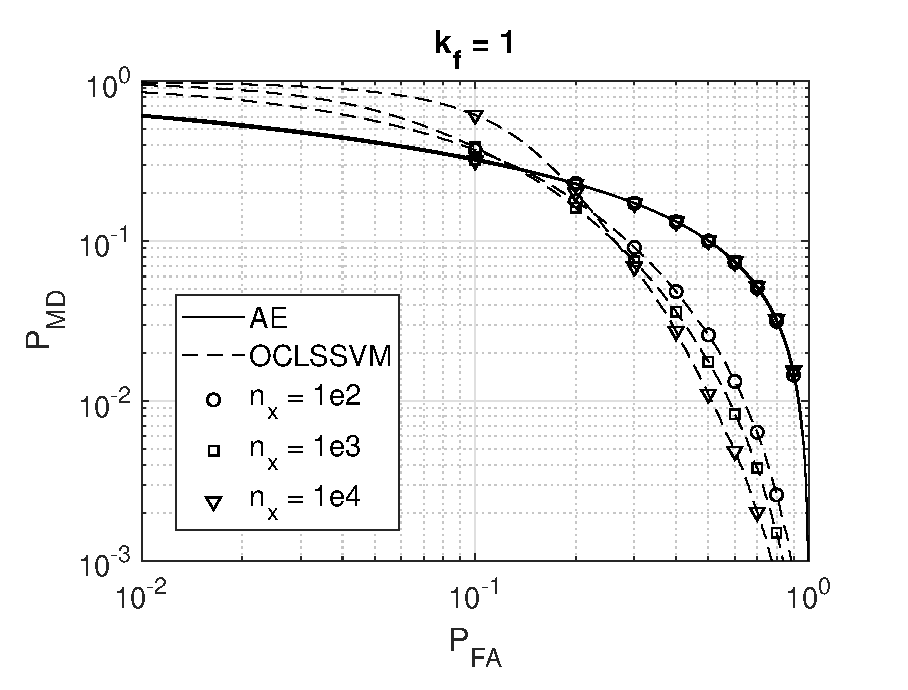
\includegraphics[width=0.6\columnwidth]{res_avgnTrain_oneClass_kf1.eps}
    \caption{\ac{roc} for one-class \acp{irlv} in a scenario with path-loss, shadowing and fading with different training set size and $k_f=1$ fading realizations,  \ac{ae} with $N_h = 2$. }
    \label{fig:kf1Oc}
\end{figure}


We now consider the effects of fading and the choice of the training points. For one-class \ac{irlv}, the training set collects only attenuation vectors from \ac{ue} located in $\mathcal{A}_0$, whereas the testing set comprises attenuation vectors of \acp{ue} both inside and outside $\mathcal A_0$. We consider $S = n_x \cdot k_f$ training points with $n_x$ locations and $k_f$ fading realizations per location. Fig.s \ref{fig:kf1Oc} and \ref{fig:kf10Oc} show the \ac{roc} for one-class \acp{irlv} systems for $k_f = 1$ and $10$, respectively. In particular \ac{oclssvm} and  \ac{ae} with $N_h=2$ are considered.  We first notice that the \ac{ae} is less sensitive to the training set size $S$. Furthermore we note that for $P_{\rm FA} > 10^{-1}$ the \ac{oclssvm} attains a lower  $P_{\rm MD}$. Moreover, we note that \ac{ae} is less sensitive to fading, as error probabilities are very similar in both figures. Instead we notice that  \ac{oclssvm} is more sensitive to fading for small values of $S$, while for a large $S$, performance get close for both values of $k_f$. Furthermore we notice that for small $S$ it is better to use one fading realization per space point ($k_f=1$) in building the training set for the \ac{oclssvm}. This is different  from what we observed for two-class classification, where taking more fading measures provided an advantage.  

If we compare Fig.s \ref{fig:kf10} and \ref{fig:kf1Oc}, we can observe that, in the considered scenario, the two-class \acp{irlv} outperform the one-class \ac{irlv}: the former achieves a lower $P_{\rm MD}$ for the same $P_{\rm FA}$, although the difference between the performance of the two methods is small. This result is expected since the two-class \ac{irlv} also exploits the (estimated) statistics of attacks, which are instead not exploited by the one-class solution. Note that, in this case, the attacker is behaving as expected by the network in the training phase, so that two-class approach is more powerful in the hypothesis testing, actually is optimum  as we shown its convergence to the \ac{np} test performance (\hl{rileggere ultima frase. giorgio}).
 
 
 

\begin{figure}[t]
    \centering
    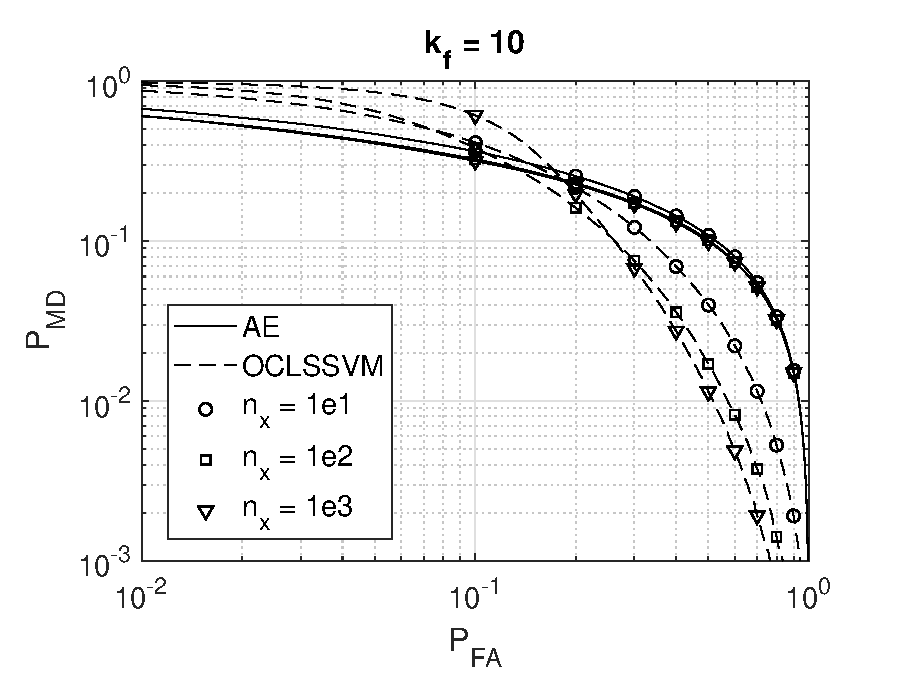
\includegraphics[width=0.6\columnwidth]{res_avgnTrain_oneClass_kf10.eps}
    \caption{\ac{roc} for one-class \acp{irlv} in a scenario with path-loss, shadowing and fading with different training set size and $k_f=10$ fading realizations,  \ac{ae} with $N_h = 2$. }
    \label{fig:kf10Oc}
\end{figure}




\begin{figure}[t]
    \centering
    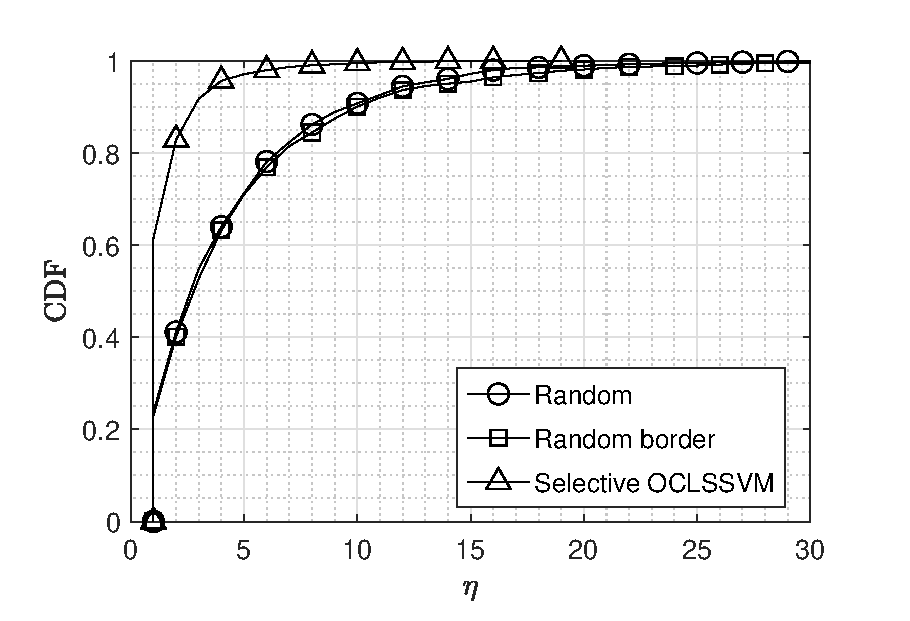
\includegraphics[width=0.6\columnwidth]{res_selective_SVM.eps}
    \caption{\ac{cdf} of the time of first successful attack $\eta$ for various attack strategies. Both the selective \ac{ml} attack  and \ac{irlv} are based on \ac{oclssvm} and $P_{\text{FA}}= 10^{-2}$.}
    \label{fig:selectiveSVM}
\end{figure}

\begin{figure}[t]
    \centering
    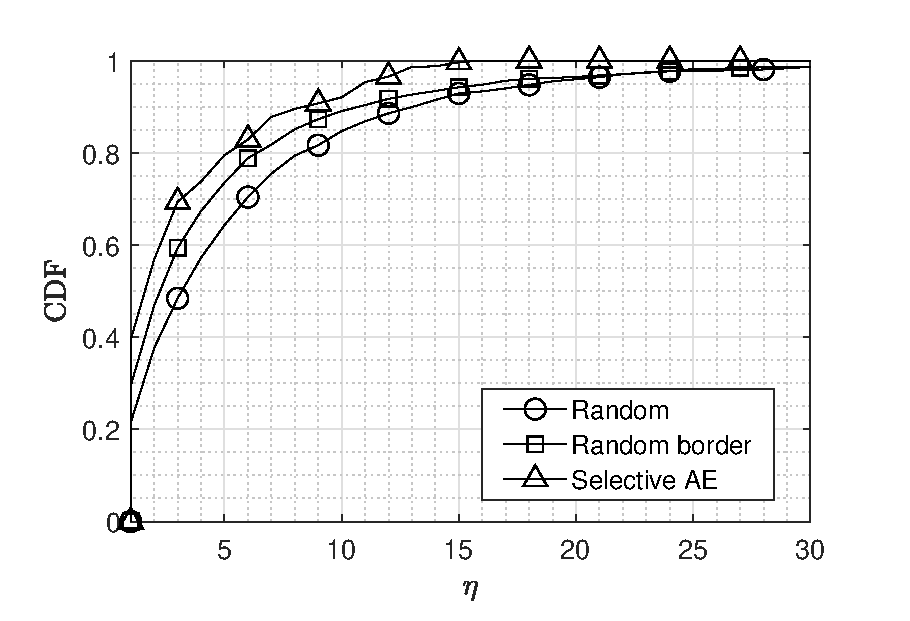
\includegraphics[width=0.6\columnwidth]{res_selective_AE.eps}
    \caption{\ac{cdf} of the time of first successful attack $\eta$ for various attack strategies. Both the selective \ac{ml} attacks  and \ac{irlv} are based on \ac{ae} and $P_{\text{FA}}= 0.5$.}
    \label{fig:selectiveAE}
\end{figure}


\subsection{\ac{ml} Attack Strategies}

We consider now the \ac{ml} attack strategies described in Section \ref{sec:attack} for the scenario of Fig. \ref{fig:mBS} and channels including path-loss, shadowing and fading. The \ac{irlv} is also implemented with one-class classifiers. 

%In order to test the attacks we set the \ac{fa} probability at the defense side, such that the threshold value needed for classification is given. We compare attacks and defense both implemented via \ac{ae} and \ac{oclssvm}. 

We compare the \ac{ml} attack strategies with uniformly random attacks, wherein attacks are launched by uniform randomly selected positions in the \ac{roi}-complementary area $\mathcal{A}_1$.  Moreover, as a na\"ive enhancement, we consider a \emph{random-border} attack, wherein the attacker moves only along a strip of 2.5 meters at the border between areas $\mathcal{A}_0$ and $\mathcal A_1$. In this way, we expect that the chances of a successful attack increase by being closer to the \ac{roi}. In this case, we assume that the \ac{roi} $\mathcal A_0$ coincides with the whole south-west building of Fig. \ref{fig:trueMap}. Therefore, on the border between $\mathcal A_0$ and $\mathcal A_1$, the \ac{ue} is on the streets and has a \ac{los} propagation characteristic, whereas region $\mathcal A_0$ has a no-\ac{los} propagation characteristic. 

The same one-class \ac{ml} algorithm is implemented both for attack and \ac{irlv}, although the attacker training set includes only points in $\mathcal A_1$, while the \ac{ap} network training set includes only  points in $\mathcal A_0$. For  \ac{irlv}  we set $k_f=10$.

Fig.s \ref{fig:selectiveSVM} and \ref{fig:selectiveAE} show the \ac{cdf} of the number of the first successful attack $\eta$ for the random, random-border and selective ML attack strategies. Fig. \ref{fig:selectiveSVM} presents results for \ac{irlv} with $P_{\rm FA}=10^{-2}$ and \ac{ml} approaches based on \ac{oclssvm}. In this case, the selective-ML attack is faster than pure random attack, which in turn perform similarly to the border-random  attack.  Fig. \ref{fig:selectiveAE}, instead, shows results for  \ac{irlv} $P_{\rm FA} =0.5$ and \ac{ml} approaches based on \acp{ae}. We observe that the random-border attack outperforms a purely random attack, while still being less-powerful than selective \ac{ml}. 

We can conclude that the \ac{ml} selective attack is clearly reducing the time to reach a success with respect to random attacks. Moreover, \ac{ae} is more robust to attacks than \ac{oclssvm} when used for \ac{irlv}, as for \ac{ae} the first successful attack as a similar statistics to random attacks while for \ac{oclssvm} the \ac{ml} selective strategy is  successful much earlier than the random strategies. 



\section{Conclusions}

In this paper, we have proposed innovative solutions for the \ac{irlv} in wireless networks that exploit the features of the channels between the \ac{ue} whose location must be verified by a trusted network of \acp{ap}. By observing that in typical situations the channel statistics are not available for \ac{irlv}, we have proposed \ac{ml}-based solutions, operating with both one- and two-class classification, i.e., with and without a-priori assumptions on attack statistics. For two-class classification we have proved that  both \ac{nn} and \ac{svm} solutions  are the most powerful tests for a given sensitivity, i.e., they are equivalent to the \ac{np} test. Instead, for one-class classification both \ac{ae} and \ac{svm} solutions are not equivalent to the \ac{glrt}. From numerical results we conclude that \ac{ml} converges to optimal performance with much smaller training set sizes than \ac{np} test implemented with estimated channel statistics. We have also investigated how to collect the training points for training in order to be robust against the channel fading.

\section*{Appendix}

	Given a finite  attenuation vector alphabet $\mathcal C = \{\bm{\alpha}_1, \ldots, \bm{\alpha}_M\}$ of $M$ elements, with $\bm{a}^{(i)} \in \mathcal C$, we indicate with $p_{\bm{a}^{(i)},t_i}(\bm{\alpha}_j, t)$, with $t \in \{-1,1\}$, the joint probability of input vector $\bm{a}^{(i)}$ and corresponding output $t_i$, $i=1, \ldots, S$.
	
	By the Glivenko–Cantelli theorem we have that with probability 1 as $S\rightarrow \infty$ there are $Sp_{\bm{a}^{(i)},t_i}(\bm{\alpha}_j,t)$ training vectors $\bm{\alpha}_j$ with associated true value $t$ in any training sequence.
	All these training points will have the same value $e_i$, from (\ref{eq:stpart}), that will appear $Sp_{\bm{a}^{(i)},y_i}(\bm{\alpha}_j,t)$ times in the sum $\sum_{i=1}^{S} e_i^2$.
	Note that in the training ensemble there could be two equal instances $\bm{a}^{(m)}=\bm{a}^{(n)}=\bm{\alpha}_j$, but with different labels $t_m \neq t_n$. Therefore, for $\bm{a}^{i}=\bm{\alpha}_j$ we can have two possible values for $e_i$, depending on $y_i$, and we denote them with $e_{j,1}$ and $e_{j,-1}$.
	This translates in only $2M$ \textit{distinct} constraints of the type \eqref{eq:stpart}.
	Asymptotically, for $S \to \infty$, problem (\ref{eq:lssvm}) becomes
	\begin{subequations}
		\label{eq:lssvm22}
		\begin{equation}
		\label{eq:lssvm2}
		\underset{\bm{w},e}{\text{min}} \quad f_l' \triangleq \frac{1}{2} \bm{w}^T \bm{w} + C S \frac{1}{2} \sum_{j=1}^M [p_{\bm{a}^{(i)},t_i}(\bm{\alpha}_j,1) e_{j,1}^2 + p_{\bm{a}^{(i)},y_i}(\bm{\alpha}_j,-1) e_{j,-1}^2]  
		\end{equation}
		subject to 
		\begin{equation}
		\label{eq:stpart2}
		[\bm{w}^T \phi (\bm{\alpha}_j) + b] = 1- e_{j,1}\quad j = 1 ,\dots,M.
		\end{equation}
		\begin{equation}
		\label{eq:stpart3}
		\quad  -[\bm{w}^T \phi (\bm{\alpha}_j) + b] = 1- e_{j,-1}\quad j = 1 ,\dots,M.
		\end{equation}
	\end{subequations}
	whose solution provides the convergence value (in probability) of vector $\bm{w}$. We write the Lagrangian
	\begin{equation}
	\mathcal{L}_1 = f_l' - \sum_{k=1}^{M} v_k \left[ \bm{w}^T \phi (\bm{\alpha}_j) + b - 1 + e_{j,1} \right] 
	- \sum_{k=1}^{M} u_k \left[- \bm{w}^T  \phi (\bm{\alpha}_j) - b  - 1 + e_{j,-1} \right], 
	\end{equation}
	where $\{u_k,v_k\}_{k=1}^{M}$ are the Lagrangian multipliers. Let us set to zero the derivatives with respect to $\{\bm{w},b,e_{j,1},e_{j,-1}, v_j,u_j\}$
	\begin{subequations}
		\begin{equation}
		\label{eq:deriv1_1}
		\frac{\partial \mathcal{L}_1}{ \partial \bm{w}}: \quad \bm{w} = \sum_{k=1}^{M} (u_k - v_k) \phi (\bm{\alpha}_k),
		\end{equation}
		\begin{equation}
		\label{eq:deriv1_2}
		\frac{\partial \mathcal{L}_1}{\partial b}: \quad \sum_{k=1}^{M} (u_k - v_k) = 0 ,
		\end{equation}
		\begin{equation}
		\label{eq:deriv1_3}
		\frac{\partial \mathcal{L}_1}{\partial e_{j,1}}: \quad v_j = CSp_{\bm{a}^{(i)},t_i}(\bm{\alpha}_j,1) e_{j,1} \quad j=1\dots M,
		\end{equation}
		\begin{equation}
		\label{eq:deriv1_4}
		\frac{\partial \mathcal{L}_1}{\partial e_{j,-1}}: \quad u_j = CSp_{\bm{a}^{(i)},t_i}(\bm{\alpha}_j,-1) e_{j,-1} \quad j=1\dots M,
		\end{equation}
		\begin{equation}
		\label{eq:deriv1_5}
		\frac{\partial \mathcal{L}_1}{\partial v_j}: \quad \bm{w}^T \phi (\bm{\alpha}_j) + b - 1 + e_{j,1} = 0 \quad j=1\dots M,
		\end{equation}
		\begin{equation}
		\label{eq:deriv1_6}
		\frac{\partial \mathcal{L}_1}{\partial u_j}: \quad - \bm{w}^T \phi (\bm{\alpha}_j) - b - 1 + e_{j,-1} = 0 \quad j=1\dots M.
		\end{equation}
	\end{subequations}
	Substituting \eqref{eq:deriv1_1}, \eqref{eq:deriv1_3} and \eqref{eq:deriv1_4} in \eqref{eq:deriv1_5} and \eqref{eq:deriv1_6} we get the system of equations
	\begin{subequations}
		\label{eq:system1}
		\begin{equation}
		\sum_{k=1}^{M} (u_k - v_k) k(\phi (\bm{\alpha}_k,\bm{\alpha}_j)) + b - 1 + \frac{v_j}{CSp_{\bm{a}^{(i)},t_i}(\bm{\alpha}_j,1)} = 0
		\quad j=1\dots M
		\end{equation}
		\begin{equation}
		- \sum_{k=1}^{M} (u_k - v_k) k(\phi (\bm{\alpha}_k,\bm{\alpha}_j)) - b - 1 + \frac{v_j}{CSp_{\bm{a}^{(i)},t_i}(\bm{\alpha}_j,-1)} = 0
		\quad j=1,\dots, M
		\end{equation}
		\begin{equation}
		\sum_{k=1}^{M} (u_k - v_k) = 0.
		\end{equation}
	\end{subequations}
	\eqref{eq:system1} is a system with $2M + 1$ equations, linear in the $2M + 1$ unknowns $\{u_k,v_k,b\}_{k=1}^{k=M}$ and therefore has finite solution. In particular, using \eqref{eq:deriv1_1}, we have
	\begin{equation}
	\label{eq:wSolution}
	\bm{w}^T\bm{w} =  \sum_{k=1}^{M} \sum_{h=1}^{M} k(\bm{\alpha}_k,\bm{\alpha}_h) (v_kv_h + u_ku_h -2 v_ku_h),
	\end{equation}
	where we used the fact that the kernel function
	\begin{equation}
	k(\bm{\alpha}_k,\bm{\alpha}_h) \triangleq \phi(\bm{\alpha}_k) \phi(\bm{\alpha}_h)^T
	\end{equation}
	 is symmetric \wrt its inputs. 
	
%	Note that while the original problem \eqref{eq:lssvm}, as $S \to \infty$, has infinite constraints, the equivalent formulation \eqref{eq:lssvm22} includes a finite number $2M$ of constraints.
	
	We conclude that $\bm{w}$ has a finite norm since the right hand side of \eqref{eq:wSolution} is a finite sum.
	  


%\bibliographystyle{IEEEtran}
%\bibliography{bibliography.bib}
\renewcommand*{\bibfont}{\footnotesize}

\printbibliography

\clearpage
\section*{Answer to Reviewers' Comments}
\section*{Reviewer: 1}

~

\setstretch{1.0}

\begin{framed}
 {\bf Rev: Positives:

- Classic hypothesis test is added on with machine learning algorithms, which bring novel ideas to the field.

- Some theories are also derived for the proposed algorithms.

- Numerical parts are solid and have many interesting insights. 

- The citations are sufficient. But there are many recent related work with machine learning in detection.
}
\end{framed}

\setstretch{1.5}

{\bf Ans:} We would like to thank the reviewer for his/her positive comments. We have addressed all the issues, updated the manuscript, and provided here a point-to-point response.  


\setstretch{1.0}
\vspace{5mm} %5mm vertical space
\begin{framed}
{\bf Rev: The machine learning part looks trivial and too classic. Much more advance schemes are available everyday on the market.}
\end{framed}
 
\setstretch{1.5}

{\bf Ans:} We agree with you that various solutions have been considered in the literature for classification. Still, we believe that the addressed problem in this paper is simple (we only need to decide between two hypotheses) and the structure/type of input is also simple (we focus on the received signal power at various base stations). Therefore, we focused on two classical approaches, i.e., neural network and support vector machines. Moreover, the intent of the paper was also to establish a strong connection between the machine learning approach -- to be used when statistics of input data in the two hypotheses is not known a priori,-- and the Neyman-Pearson test, to be used when the statistics are known. In this respect, the presented theoretical results fill the gap and are actually applicable also to more complex scenarios. Indeed, as we consider the neural network as a generic parametric function, whose parameters are updated using specific target function, our results extend for example also to deep learning solutions, using more complex neural networks.

In order to make this point more clear we have updated the Introduction, by extending the literature survey, and adding the following sentence:
\begin{quote}
    "\revp{rev11a}"
\end{quote}

Moreover, we have added the following sentence after Theorem 1, to indicate that it also pertains quite complex deep-learning NNs:
\begin{quote}
    "\revp{rev11b}"
\end{quote}
 
Lastly, numerical results have been revised and now include the performance of more complex scenarios, using both more \acp{ap} (thus increasing the input size of the machine) and using more complex deep-learning \acp{nn}. 

\setstretch{1.0}
\vspace{5mm} %5mm vertical space
\begin{framed}
\noindent {\bf Rev:
Theorem 1 looks too obvious.}
\end{framed}

\setstretch{1.5}
{\bf Ans:} Although Theorem 1 (Corollary 1 in the new version of the manuscript) largely relies on an existing result that connects the MLP to the Bayes optimal discriminant function, it is not so common in journal and even books on ML to frame the classification problem as a hypothesis testing problem and investigate the connection between ML solutions and Neyman-Pearson optimal test. We believe that this is the contribution of Theorem 1, also the other theorems of the manuscript that extended this results to SVM solutions and various training options. Following your advice we have here briefly recalled the result of \cite{Ruck-90} and reduced to the minimum the derivations for the proof of Theorem 1, which now only presented as a corollary of the result of \cite{Ruck-90}.

\setstretch{1.0}
\vspace{5mm} %5mm vertical space
\begin{framed}
\noindent {\bf Rev:
Neural networks in Figure 2 (Fig. \ref{fig:aeArch} in the new version of the manuscript) are fully connected and kind of shallow.}
\end{framed}

\setstretch{1.5}
{\bf Ans:} \hl{CAMBIARE LA FIG. 3!!!} We thank the reviewer for his/her comment. We have modified Fig. \ref{fig:aeArch} including the possibility of \hl{not having some connections among neurons}. We also added the following more extensive description of the AE:
\begin{quote}
    "\revp{deep ae}"
\end{quote}
Moreover, following the advice of another reviewer, we have included more hidden layers in the same figure.

In the numerical results we still use a fully-connected NN (with two hidden layers), as the number of input in the considered scenario is small and still tractable with this kind of networks.

% We would like to thank the reviewer for having indicated more complex solutions to our problem. \hl{NON CAPISCO} In this paper we do not consider convolutional autoencoders and hence we implemented networks with fully connected layers. We added a more general description of the AE in Sec. \ref{sec:auto} : 
% \begin{quote}
%     "\revp{deep ae} \cite[Chapter 14]{goodfellow}.
%     \revp{deep ae2} \cite[Chapter 14]{goodfellow}."
    
% \end{quote}
 
\setstretch{1.0}
\vspace{5mm} %5mm vertical space
\begin{framed}
\noindent {\bf Rev:
Abstract sounds to stress something like the attacks, while in the main text, it is rarely mentioned and discussed.}
\end{framed}

\setstretch{1.5}
{\bf Ans:} Thanks for your comment. We have revised the abstract to avoid misunderstanding about the attacks. It now reads as follows:
\begin{quote}
    "\revp{rev14}"
\end{quote}

\clearpage 
\section*{Reviewer: 2}
~
\setstretch{1.0}

\begin{framed}
\noindent {\bf Rev:
There exist a large number of literature on location aware services in WiFi as well as cellular networks. It must be clearly described what the benefits of the proposed (simple and idealised hypothesis test approach) are.}
\end{framed}

\setstretch{1.5}
{\bf Ans:} \hl{TBD}

\setstretch{1.0}
\vspace{5mm} %5mm vertical space
\begin{framed}
\noindent {\bf  Rev: In the numerical simulations a comparison with state of the art algorithms should be included.}
\end{framed}

\setstretch{1.5}
{\bf Ans:} Thank you for the suggestion. In the revised manuscript we have included the description of a literature method, wherein first the position of the user is estimated and then compared with the area of interest. Most of the literature assumes a perfect estimate of the position, thus trivially solving the \ac{irlv} problem. We have extended this approach taking into account estimation errors. The comparison method is briefly described in Section \ref{seccomp} as
\begin{quote}
    "\revp{literature_1} 
	\begin{align}
 \hat{\bm x}_{\rm UE} =  \underset{\bm x}{\arg \min} \sum_{n=1}^{N_{\rm AP}} \left(L(\bm{x},\bm{x}_{\rm AP}^{(n)}) - L(\bm{x}_{\rm UE},\bm{x}_{\rm AP}^{(n)}) \right)^2,\label{probmindist}
\end{align}
\revp{literature_2}
$$
\hat{\mathcal{H}}_{\rm MMSE} = 
\begin{cases}
\mathcal{H}_0 \quad \text{if } d < d_0 \\
\mathcal{H}_1 \quad {\rm otherwise}.
\end{cases}
$$
\revp{literature_3}"
\end{quote}

Moreover, Fig \hl{TBD} ... now include the comparison with the literature model. We have added the following comments on the figures: \hl{TBD}

\setstretch{1.0}
\vspace{5mm} %5mm vertical space
\begin{framed}
\noindent {\bf Rev:
The quality of the graphics could be improved.}
\end{framed}

\setstretch{1.5}
{\bf Ans:} Thank you for pointing out this issue. We have revised all the graphics in the paper and improve their quality.

\setstretch{1.0}
\vspace{5mm} %5mm vertical space
\begin{framed}
\noindent {\bf Rev:
The asymptotic results are only available for very idealised cases.}
\end{framed}

\setstretch{1.5}
{\bf Ans:} As asymptotic results were shown in comparison with the \ac{np} framework described in Section \ref{sec:los}, we revised the entire Section in order to include more realistic scenarios and show the effect of the different channel parameters on the \ac{irlv} performance. In particular we added in Section \ref{sec:los}
\begin{quote}
"\revp{simpleScen}

\revp{simpleScen2}
\begin{equation*}
p(a|\mathcal{H}_0) = \int_{0}^{R_{\rm in}} p\left( \frac{P_{\rm tx}}{a} | d = d_0\right)p(d_0| d_0 \in \mathcal{A}_0) \, dd_0,   
\end{equation*}
\revp{simpleScen2_1}
\begin{equation*}
p(d_0| d_0 \in \mathcal{A}_0) =
\begin{cases}
\frac{2 d_0}{R_{\rm in} ^ 2-R_{\rm min}^2} \, \, d_0 \in [R_{\rm min}, R_{\rm in}], \\
0 \, \, d_0 > R_{\rm in}
\end{cases}
\end{equation*}
\revp{simpleScen2_2}
\begin{equation*}
p(d_0| d_0 \in \mathcal{A}_1) =
\begin{cases}
0 \, \, d_0 \leq R_{\rm in},\\
\frac{2 d_0}{R ^ 2- R_{\rm in} ^2} \, \, d_0 \in (R_{\rm in},R].
\end{cases}
\end{equation*}
1) \emph{Fading scenario}
\revp{simpleScen3}
\begin{equation*}
    p(a|\mathcal{H}_0) = 
    \frac{2}{R_{\rm in}^2-R_{\rm min}^2}\int_{R_{\rm min}}^{R_{in}} 10^{P_{{\rm PL},{\rm LOS}}(d_0)/10} \exp\left(-10^{P_{{\rm PL},{\rm LOS}}(d_0)/10} \frac{P_{\rm tx}}{a}\right)d_0 \, dd_0,
\end{equation*}
\revp{simpleScen3_1}
\begin{equation*}
    p(a|\mathcal{H}_1) = 
    \frac{2}{R^2-R_{\rm in}^2}\int_{R_{\rm in}}^R 10^{P_{{\rm PL},{\rm LOS}}(d_0)/10} \exp\left(-10^{P_{{\rm PL},{\rm LOS}}(d_0)/10} \frac{P_{\rm tx}}{a}\right)d_0 \, dd_0,
\end{equation*}
\revp{simpleScen3_2}
\begin{equation*}
   \mathcal{M}(a) =
   \ln\left(\frac{R^2-R_{\rm min}^2}{R_{\rm in}^2-R_{\rm in}^2}\frac{\mathcal{V}(R_{\rm min},a)-\mathcal{V}(R_{\rm in},a)}{\mathcal{V}(R_{\rm in},a)-\mathcal{V}(R,a)}\right),
\end{equation*}
\revp{simpleScen3_2_1}
\begin{equation*}
\mathcal{V}(d_0,a) = \exp\left(-\frac{P_{\rm tx}}{a}\left(\frac{4 \pi f_0 d_0}{c}\right)^2\right) \left(\frac{P_{\rm tx}}{a}\left(\frac{4 \pi f_0 d_0}{c}\right)^2+1\right) .   
\end{equation*}
\revp{simpleScen3_3}
\begin{equation*}
 \mathcal{M}(a) =
 \ln\left(\frac{R^2-R_{\rm in}^2}{R_{\rm in}^2-R_{\rm min}^2}\frac{\Gamma\left(\frac{5}{3},\frac{P_{\rm tx}}{a}\left(\frac{4 \pi f_0}{c}\right)^3 R_{\rm min}^3\right)-\Gamma\left(\frac{5}{3},\frac{P_{\rm tx}}{a}\left(\frac{4 \pi f_0}{c}\right)^3 R_{\rm in}^3\right)}{\Gamma\left(\frac{5}{3},\frac{P_{\rm tx}}{a}\left(\frac{4 \pi f_0}{c}\right)^3 R_{\rm in}^3\right)-\Gamma\left(\frac{5}{3},\frac{P_{\rm tx}}{a}\left(\frac{4 \pi f_0}{c}\right)^3 R^3\right)}\right),
\end{equation*}
\revp{simpleScen3_4}


2) \emph{Shadowing scenario}
\revp{simpleScen4}
\begin{equation*}
   p(a|\mathcal{H}_0) = 
    \frac{2}{R_{\rm in}^2-R_{\rm min}^2}\int_{R_{\rm min}}^{R_{\rm in}} \exp\left(-\frac{1}{2}\frac{\left(\frac{P_{\rm tx}}{a}+10\nu\log_{10}\left(\frac{4 \pi f_0 d_0}{c}\right)\right)^2}{\sigma_s^2}\right) d_0 \, d d_0,  
\end{equation*}
\revp{simpleScen4_1}
\begin{equation*}
    p(a|\mathcal{H}_1) = 
    \frac{2}{R^2-R_{\rm in}^2}\int_{R_{\rm in}}^R \exp\left(-\frac{1}{2}\frac{\left(\frac{P_{\rm tx}}{a}+10\nu\log_{10}\left(\frac{4 \pi f_0 d_0}{c}\right)\right)^2}{\sigma_s^2}\right) d_0 \, d d_0 .
\end{equation*}
\revp{simpleScen4_2}
\begin{equation*}
    \mathcal{M}(a) = \ln\left(\frac{R^2}{R_{\rm in}^2} \frac{\mathcal{T}(R_{\rm in})-\mathcal{T}(R_{\rm min})}{\mathcal{T}(R)-\mathcal{T}(R_{\rm in})}\right),
\end{equation*}
\revp{simpleScen4_3}
\begin{equation*}
    \mathcal{T}(d_0) = \erf\left( \frac{\frac{100 \nu^2}{\sigma_s^2}\ln(d_0)-\ln^2(10)+\frac{\frac{P_{\rm tx}}{a} 10 \nu \ln(10)}{2\sigma_s^2}}{\sqrt{1/2\sigma_s^2}10\nu\ln(10)}\right),
\end{equation*}
\revp{simpleScen4_4}"
\end{quote}

Then we showed the convergence of all the \ac{ml}-based systems to the optimal \ac{np} framework in Sec. \ref{sec:singleAp}.

\setstretch{1.0}
\vspace{5mm} %5mm vertical space
\begin{framed}
\noindent {\bf Rev:
An overall framework/unified model is missing. The impact of the paper would be much larger if the model-less learning based approach is tested with real experimental data.}
\end{framed}

\setstretch{1.5}
{\bf Ans:} \hl{TBD}

\setstretch{1.0}
\vspace{5mm} %5mm vertical space
\begin{framed}
\noindent {\bf Rev:
The security attack by choosing locations is not properly modelled and does not contain a complete analysis and assessment. Either elaborate or do not include. If the security attack is included, please modify the title accordingly.}
\end{framed}

\setstretch{1.5}
{\bf Ans:} Indeed, we do not have the ambition to fully describe an attack in which the user chooses the location. In order to make this point more clear we have revised the abstract to avoid misunderstanding about the attacks. It now reads as follows:
\begin{quote}
    "\revp{rev14}"
\end{quote}

\setstretch{1.0}
\vspace{5mm} %5mm vertical space
\begin{framed}
\noindent {\bf Rev:
There are a number of typos and English grammar mistakes. The paper should be carefully proofread.}
\end{framed}

\setstretch{1.5}
{\bf Ans:} Thank you for pointing out this issue. We have carefully revised the paper to avoid typos and grammar mistakes.

\setstretch{1.0}
\vspace{5mm} %5mm vertical space
\begin{framed}
\noindent {\bf Rev:
Most applications are from the WiFi or IoT area. Why the paper then studies the cellular setup?}
\end{framed}

\setstretch{1.5}
{\bf Ans:} We agree with you that \ac{irlv} has been studied for WiFi applications. Still, we believe that the problem will be also relevant for future cellular networks that may provide IoT services and will rely more and more on the position of the user for location-specific services. On this point we have added the following sentence in the Introduction:
\begin{quote}
    "\revp{WiFi}"
\end{quote}
Moreover, in Section II we have added the following sentence:
\begin{quote}
    "\revp{WiFi2}"
\end{quote}
\setstretch{1.0}
\vspace{5mm} %5mm vertical space
\begin{framed}
\noindent {\bf Rev:
If books are referenced, please include page or section or Theorem numbers for easier reference.}
\end{framed}

\setstretch{1.5}
{\bf Ans:} Thank you for the suggestion. We revised the manuscript in order to include chapter numbers for the cited books.

\setstretch{1.0}
\vspace{5mm} %5mm vertical space
\begin{framed}
\noindent {\bf Rev:
In the introduction, there are no SoA references for the security attacks including models and countermeasures.}
\end{framed}

\setstretch{1.5}
{\bf Ans:} Ans

\setstretch{1.0}
\vspace{5mm} %5mm vertical space
\begin{framed}
\noindent {\bf Rev:
Fig. 1 is not adding any real value. Please add more information like showing the variables such as regions A0 and A1 and the channel parameters.}
\end{framed}

\setstretch{1.5}
{\bf Ans:} Thank you for pointing out this issue. We revised Fig. 1 with system parameters.
\setstretch{1.0}

\vspace{5mm} %5mm vertical space
\begin{framed}
\noindent {\bf Rev:
Justify and motivate why only the receive power and not the phase is used for hypothesis test.}
\end{framed}

\setstretch{1.5}
{\bf Ans:} The received power was considered only as an example of channel feature that can be exploited for \ac{irlv}, and definitely other options as the phase or the wideband impulse response can be used for localization. In order to make this point more clear we added the following sentence in Section II:
\begin{quote}
    "\revp{revPHASE}"
\end{quote}
\setstretch{1.0}



\vspace{5mm} %5mm vertical space
\begin{framed}
\noindent {\bf Rev:
Provide a reference for the chosen shadowing correlation model below (4).}
\end{framed}

\setstretch{1.5}
{\bf Ans:} We added the reference to \cite[Chapter 2.7]{goldsmith2005} after the description of the shadowing correlation.

\setstretch{1.0}
\vspace{5mm} %5mm vertical space
\begin{framed}
\noindent {\bf Rev:
Explain how to choose the parameter Lambda in (6).}
\end{framed}

\setstretch{1.5}
{\bf Ans:} Thank you for pointing out this. We added in Sec. \ref{sec:auth}
\begin{quote}
"\revp{lambda}"
\end{quote}

\setstretch{1.0}
\vspace{5mm} %5mm vertical space
\begin{framed}
\noindent {\bf Rev:
Provide more details on $\zeta(\rho)$ below (8) and its operational meaning.}
\end{framed}

\setstretch{1.5}
{\bf Ans:} As the provided example in the old version of the paper was not practical from an operational point of view we modified it by considering two different scenarios: the former affected by path-loss and fading and the latter affected by path-loss and shadowing. The parameter $\zeta(\rho)$ does not exist anymore, as also the overall scenario for the example of application of the \ac{np} lemma has been changed, as shown in Fig. \ref{fig:simpScen}. 

\setstretch{1.0}
\vspace{5mm} %5mm vertical space
\begin{framed}
\noindent {\bf Rev:
The example closes with equation (11): How does the test function look like? What are the insights from this example?}
\end{framed}

\setstretch{1.5}
{\bf Ans:} We decided not to include the plots for the test functions (\ref{eq:llr1}), (\ref{eq:llr2}) and (\ref{eq:llr3}) as they do not provide any insights if not compared with the threshold value $\Lambda$, allowing us to state whether the tested received power comes from a user located in $\mathcal{A}_0$ or $\mathcal{A}_1$. From this example we get the closed form equation of the functions that allows us to classify the received power in an optimal way, i.e., providing the minimum $P_{\rm MD}$ for a given $P_{\rm FA}$. In order to clarify this, we added in Sec. \ref{sec:los}:
\begin{quote}
"\revp{llrComp}"
\end{quote}

\setstretch{1.0}
\vspace{5mm} %5mm vertical space
\begin{framed}
\noindent {\bf Rev:
Section III, explicitly state that you apply supervised learning.}
\end{framed}

\setstretch{1.5}
{\bf Ans:} Thank you for the suggestion. We added in Sec \ref{sec:irlvML}
\begin{quote}
"\revp{supervised}"
\end{quote}

\setstretch{1.0}
\vspace{5mm} %5mm vertical space
\begin{framed}
\noindent {\bf Rev:
Below (13), is $\lambda$ optimised with ML, too?}
\end{framed}

\setstretch{1.5}
{\bf Ans:} Since Theorems 1 and 2 hold, the hypothesis testing implemented by the \ac{nn} classifier is the same implemented by the \ac{np} framework. Therefore the parameter $\lambda$ does not need to be optimize, but instead guarantees the minimum $P_{\rm MD}$ for the chosen $P_{\rm FA}$. In order to clarify this points we added in Sec. \ref{sec:nn}:
\begin{quote}
"\revp{lambdaNN}"
\end{quote}

\setstretch{1.0}
\vspace{5mm} %5mm vertical space
\begin{framed}
\noindent {\bf Rev:
Theorem 1 is basically a Corollary from [18] (now \cite{Ruck-90}).}
\end{framed}

\setstretch{1.5}
{\bf Ans:} Following your suggestion we have reported the theorem by \cite{Ruck-90} and denoted former Theorem 1 as a corollary.
\setstretch{1.0}


\vspace{5mm} %5mm vertical space
\begin{framed}
\noindent {\bf Rev:
From the flow of the paper, it is not clear, why the section on NN CE Design is needed. Furthermore, sections D and E on SVM should be merged.}
\end{framed}

In order to clarify why both \ac{mse} and \ac{ce} loss functions are considered for \acp{nn} we added in \ref{sec:nn}:
\begin{quote}
"\revp{ceNeeded}"
\end{quote}

In Sec. \ref{sec: mse_train}

\begin{quote}
"\revp{ceNeeded2}"
\end{quote}

In Sec. \ref{sec: ce_train}

\begin{quote}
"\revp{ceNeeded3} \cite[Chapter~5.2]{Bishop2006}."
\end{quote}

Furthermore we merged Sec.s D and E on \ac{svm} as suggested by the reviewer.


\setstretch{1.0}
\vspace{5mm} %5mm vertical space

\begin{framed}
\noindent {\bf Rev:
In Theorem 3 and following, the assumption of perfect training (reaching a global optimum) should be justified. Lemma 1 alone is not sufficient.}
\end{framed}

\setstretch{1.5}
{\bf Ans:} In Theorem 3 we analyze the function obtained by SVM when it converges to the global optimum. We agree with you that in general, this requires a very long training, although this condition alone is not enough to ensure convergence to the optimum. In order to make this point more clear we have rewritten the hypothesis of Theorem 3 as follows:
\begin{quote}
    "\revp{revGO}"
\end{quote}

\setstretch{1.0}
\vspace{5mm} %5mm vertical space
\begin{framed}
\noindent {\bf Rev:
The phrase "hyperparameter" is first used explicitly in Sec. 3-E without introducing it. However, it is implicitly used earlier when the activation function in NNs and kernel function in SVMs are described as being "fixed" (which refers to being a hyperparameter).}
\end{framed}

\setstretch{1.5}
{\bf Ans:} \hl{TBD}


\setstretch{1.0}
\vspace{5mm} %5mm vertical space
\begin{framed}
\noindent {\bf Rev:
Section IV switches to a new model where data is only collected within region A0. This is not clear and also not justified.}
\end{framed}

\setstretch{1.5}
{\bf Ans:} In Sec. \ref{sec:OneClass} the new model collects data uniquely from region $\mathcal{A}_0$ in the training phase and consider particular implementation of \ac{ml} classifiers able to distinguish between two classes by being trained only with samples of one class. Hence samples are collected from $\mathcal{A}_0$ during the training phase and from both $\mathcal{A}0$ and $\mathcal{A}_1$ during the testing phase. 

In order to clarify this aspect we added in Sec. \ref{sec:OneClass}:
\begin{quote}
"\revp{oneClass}"
\end{quote}

The choice of this new setting is motivated by the fact that, as reported in Sec. \ref{sec:OneClass}:
\begin{quote}
"In practice, having training points available for both regions $\mathcal A_0$ and ${\mathcal A}_1$ may be difficult since $a$) region $\A{1}$ may be quite wide and not necessarily well defined (being simply the complementary region of $\mathcal A_0$) and $b$) the attacker may use multiple antennas and, by beamforming, can induce attenuation estimates that not necessarily correspond to points in the region $\A{1}$."
\end{quote}


\setstretch{1.0}
\vspace{5mm} %5mm vertical space
\begin{framed}
\noindent {\bf Rev:
In the AE architecture, the operational meaning and benefits of the low dimensional hidden layer are not clearly derived. Furthermore, the linear activation is not motivated.}
\end{framed}

\setstretch{1.5}
{\bf Ans:} As \acp{ae} are well known architectures, the in-depth description of the meaning of the low dimensional layer as well as its derivation is beyond the scope of this paper, as well it is the choice of the linear activation function at the output layer (usual choice according to \cite[Chapter 14]{Goodfellow}). We added in Sec. \ref{sec:auto} a reference to \cite[Chapter 14]{Goodfellow}, for a more accurate description of the characteristics of \acp{ae}.

\setstretch{1.0}
\vspace{5mm} %5mm vertical space
\begin{framed}
\noindent {\bf Rev:
The resulting IRLV test function is the simple MSE thresholding.}
\end{framed}

\setstretch{1.5}
{\bf Ans:} As the \ac{ae} is trained to attempt to copy the input to its output the result is that, in the testing phase, only those vectors with the same features of the training set will be reconstructed with small \ac{mse}, whereas input vectors with features different from those of the training set will be mapped to different vectors at the output, and hence with high \ac{mse}. Since training is based on vectors collected from area $\mathcal{A}_0$ and we want to grant access to the systems only to users located inside $\mathcal{A}_0$ and hence whose vectors will have the same features of the training set, by thresholding the \ac{mse} we can obtain the classifier needed for the \ac{irlv}.

\setstretch{1.0}
\begin{framed}
\noindent {\bf Rev:
The section on the ML-based attack strategies does not have a clear model and the interaction between system and attacker are correctly detailed. It seems a non-cooperative game model could fit here.}
\end{framed}
\setstretch{1.5}
{\bf Ans:} Thank you for your observation. The previous description of the attack was confusing, as it was also mentioning various strategies. We have completely rewritten Section \ref{sec:attack}, focusing on the specific attack and stressing its motivation, while hinting to other possibile strategies. The new section reads as follows:
\begin{quote}
    "\revp{sezattack}
\begin{enumerate}
    \item The attacker visit  $N$  points spread uniformly at random outside $\mathcal A_0$. From each point it collects the attenuation vector and performs the attack. If any of the attacks is successful, the procedure is stopped.
    \item If none of the $N$ attacks has been successful, the attenuation vectors are used to train a one-class classifier.
    \item The attacker picks a new position uniformly at random outside $\mathcal A_0$ and feeds its attenuation vector to the trained classifier.
    \item If the vector is classified as belonging to the class it is discarded, and the procedure goes back to point 3), otherwise an attack from that position is performed.
    \item If the attack is successful, the procedure is stopped. Otherwise, the attenuation vector is used to as further training input of the one-class classifier and the procedure goes back to point 3).
\end{enumerate}
\revp{sezattack2} 
\end{quote}


\setstretch{1.0}
\vspace{5mm} %5mm vertical space
\begin{framed}
\noindent {\bf Rev:
Reason for using Eq. (38) as activation function for the output layer is missing, especially since it is not a common choice for an activation function. Motivate the design choices!}
\end{framed}
\setstretch{1.5}


{\bf Ans:} 
\hl{Ruvoletto}
Thanks for havigh highlighted this issue. We have carefully revised the AE and its design choice and we now use common activation functions in the literature. In particular, in Section \ref{sec:numResOneClass} we specify
\begin{quote}
"\revp{designAE}"
\end{quote}

\setstretch{1.0}
\vspace{5mm} %5mm vertical space
\begin{framed}
\noindent {\bf Rev:
Why not using more hidden layers to improve performance?}
\end{framed}

\setstretch{1.5}
{\bf Ans:} In the revised manuscript both the feedforward \acp{nn} and the \ac{ae} hev been extended to include multiple layers in order to improve the system performance as suggested by the reviewer. Results are reported in Sec. \ref{sec:numRes}.

\setstretch{1.0}
\vspace{5mm} %5mm vertical space
\begin{framed}
\noindent {\bf Rev:
A illustration of the considered layout in Sec. V-A might be helpful.}
\end{framed}

\setstretch{1.5}
{\bf Ans:} Thank you for the suggestion. We added in Sec. \ref{sec:los} Fig. \ref{fig:simpScen} to illustrate the scenario where the \ac{np} framework has been applied and for which Sec. \ref{sec:singleAp} reports the numerical results.

\setstretch{1.0}
\vspace{5mm} %5mm vertical space
\begin{framed}
\noindent {\bf Rev:
In the assessment of Fig 3 ( Fig. \ref{fig:ceVSmse} in the revised paper), the advantage of NN versus N-P should be clarified, too, since they perform equally (bad).}
\end{framed}

\setstretch{1.5}
{\bf Ans:} We added in Sec. \ref{sec:los}:
\begin{quote}
"\revp{llrComp}"
\end{quote}

Furthermore the performance of the resulting \ac{irlv} system has been improved by considering more complicated scenarios for which is possible to compute closed form solutions for the \acp{llr}.

\setstretch{1.0}
\vspace{5mm} %5mm vertical space
\begin{framed}
\noindent {\bf Rev:
The scenario in Fig. 4 (Fig. \ref{fig:map} in the revised paper) is not well motivated. Why should the region A0 be outside the two main streets?}
\end{framed}

\setstretch{1.5}
{\bf Ans:} There is no special reason for the positioning of area $\mathcal A_0$ outside of the two streets, other than considering it inside a building (e.g., an office). In order to clarify this point we added in Section \ref{sec:singleAp}:
\begin{quote}
"\revp{building}"
\end{quote}

\hl{Moreover, we consider a general position of the area...}

\setstretch{1.0}
\vspace{5mm} %5mm vertical space
\begin{framed}
\noindent {\bf Rev:
The evaluation in the end of Sec V-B sounds contradictory. First, it is said that "[...] for small S, performance get slightly worse as $k_f$ grows.". Second, at the end of the evaluation, it is stated that "[...] in practical situations where the points for training may be limited, it may be advantageous to collect more fading realization per location.". Another way of saying this would be that for small S ("limited number of training points"), the number of $k_f$ should be increased ("collect more fading realizations per location"). However, this is contradictory to the first statement, that the performance decreases with increasing $k_f$ for small S.
- The considered layout in Sec. V-C is unclear.
}
\end{framed}

\setstretch{1.5}
{\bf Ans:} \hl{TBD}

\setstretch{1.0}
\vspace{5mm} %5mm vertical space
\begin{framed}
\noindent {\bf Rev:
The conclusions from the numerical simulations (last paragraph before Section VI) are very specific and contain mainly numerical evidence from the chose numerical scenarios.}
\end{framed}

\setstretch{1.5}
{\bf Ans:} \hl{TBD}

\setstretch{1.0}
\vspace{5mm} %5mm vertical space
\begin{framed}
\noindent {\bf Rev:
In the references: check capitalised letters in [14], [20]. Check author names in [16].}
\end{framed}

\setstretch{1.5}
{\bf Ans:} Thank you for pointing out the mistakes. We have carefully revised the references section. 
\vspace{5mm} %5mm vertical space


\clearpage


\section*{Reviewer 3}


\setstretch{1.0}
\begin{framed}
\noindent {\bf Rev:
The references of the work can be further enhanced and the model descriptions are not always comprehensive. Please explain the numerical results for more details. For example, please add the benchmark scheme to convince readers. In addition, the presentation can be further improved and the complexity of the proposed scheme should be provided.}
\end{framed}

\setstretch{1.5}
{\bf Ans:} We would like to thank your for your useful suggestions. We have carefully revised the paper according to your indications, providing more explanations of the numerical results \hl{check}, improving the presentation, comparing our solutions with existing ones, and assessing the complexity of the proposed approach \hl{CHECK}.

\setstretch{1.0}
\vspace{5mm} %5mm vertical space
\begin{framed}
\noindent {\bf Rev:
Please compare the proposed scheme with other existing schemes.}
\end{framed}

\setstretch{1.5}
{\bf Ans:} Thank you for the suggestion. In the revised manuscript we have included the description of a literature method, wherein first the position of the user is estimated and then compared with the area of interest. Most of the literature assumes a perfect estimate of the position, thus trivially solving the \ac{irlv} problem. We have extended this approach taking into account estimation errors. The comparison method is briefly described in Section \ref{seccomp} as
\begin{quote}
    "\revp{literature_1} 
	\begin{align}
 \hat{\bm x}_{\rm UE} =  \underset{\bm x}{\arg \min} \sum_{n=1}^{N_{\rm AP}} \left(L(\bm{x},\bm{x}_{\rm AP}^{(n)}) - L(\bm{x}_{\rm UE},\bm{x}_{\rm AP}^{(n)}) \right)^2,\label{probmindist}
\end{align}
\revp{literature_2}
$$
\hat{\mathcal{H}}_{\rm MMSE} = 
\begin{cases}
\mathcal{H}_0 \quad \text{if } d < d_0 \\
\mathcal{H}_1 \quad {\rm otherwise}.
\end{cases}
$$
\revp{literature_3}"
\end{quote}

Moreover, Fig \hl{TBD} ... now include the comparison with the literature model. We have added the following comments on the figures: \hl{TBD}
\setstretch{1.0}
\vspace{5mm} %5mm vertical space
\begin{framed}
\noindent {\bf Rev:
Proof that this proposed scheme has robust against the channel fading. In other words, could you please provide some numerical results to support the robust of this scheme?}
\end{framed}

\setstretch{1.5}
{\bf Ans:} Please note that our considered channel model includes fading. Indeed, Fig.s \hl{lista} all include fading effect. Moreover, we have also considered a refinement of our approach, explicitly targeting the adverse effect of fading, wherein the input data to the learning machines are obtained by averaging over multiple fading realizations. By choosing the number of averaged realization we can understand the relevance of averaging fading, taking into account that having multiple realizations of attenuation vectors may not always be possibile and takes additional time. In order to make this point more clear we have added the following sentences in Section \ref{sec:auth}:
\begin{quote}
    "\revp{avg_1}
$$
a^{(n)}_{\Sigma} = \frac{1}{N_{\rm avg}}\sum_{j=1}^{N_{\rm avg}} a^{(n)}.
$$
    \revp{avg_2}"
\end{quote}


\setstretch{1.0}
\vspace{5mm} %5mm vertical space
\begin{framed}
\noindent {\bf Rev:
What are the computation complexity of the two machine learning methods (i.e., neural networks (NNs) and SVM)?}
\end{framed}

\setstretch{1.5}
{\bf Ans:} \hl{TBD}

\setstretch{1.0}
\vspace{5mm} %5mm vertical space
\begin{framed}
\noindent {\bf Rev:
The results in terms of the miss detection rate and the false alarm rate in Fig. 3 [Fig. \ref{fig:ceVSmse} in the revised paper] are not practical. Please explain.}
\end{framed}

\setstretch{1.5}
{\bf Ans:} Based on the reviewer's comments we revised Fig. \ref{fig:ceVSmse} and the relative theoretical part in Sec. \ref{sec:los}. Results show that the implemented system achieves petter performance and the equivalence between hypothesis testing based on the \ac{np} framework and via \ac{ml} is still verified.

\vspace{5mm} %5mm vertical space

\setstretch{1.0}
\vspace{5mm} %5mm vertical space
\begin{framed}
\noindent {\bf Rev:
A couple of papers are worth citing:

(1). Physical layer authentication over MIMO fading wiretap channels, IEEE Trans. Wireless Communications, 2012.

(2). PHY-layer spoofing detection with reinforcement learning in wireless networks, IEEE Trans. Vehicular Technology,2016.
}
\end{framed}

\setstretch{1.5}
{\bf Ans:} We have added a citation of the two papers in the Introduction, within the following sentence:
\begin{quote}
    "\revp{rev3cit}"
\end{quote}

\end{document}
